% \documentclass[lineno,twocolumn,endfloat,biblatex]{biophys-new}
%%%%%%%%%%%%%%%%%%%%%%%%%%%%%%%%%%%%%%%%%%%%%%%%%%%%%%%%%%%%
%%% LIVECOMS ARTICLE TEMPLATE FOR BEST PRACTICES GUIDE
%%% ADAPTED FROM ELIFE ARTICLE TEMPLATE (8/10/2017)
%%%%%%%%%%%%%%%%%%%%%%%%%%%%%%%%%%%%%%%%%%%%%%%%%%%%%%%%%%%%
%%% PREAMBLE
\PassOptionsToPackage{prologue,dvipsnames}{xcolor}
\documentclass[9pt,tutorial]{livecoms}
% Use the 'onehalfspacing' option for 1.5 line spacing
% Use the 'doublespacing' option for 2.0 line spacing
% Use the 'lineno' option for adding line numbers.
% Use the 'pubversion' option for adding the citation and publication information to the document footer, when the DOI is assigned and the article is added to a live issue.
% The 'bestpractices' option for indicates that this is a best practices guide.
% Omit the bestpractices option to remove the marking as a LiveCoMS paper.
% Please note that these options may affect formatting.

\usepackage{lipsum} % Required to insert dummy text
\usepackage[version=4]{mhchem}
\usepackage{siunitx}
\DeclareSIUnit\Molar{M}
\usepackage[italic]{mathastext}
\graphicspath{{figures/}}
\usepackage{amsmath}
\usepackage{hyperref}
\usepackage{verbatim}

% use special package to label equations for funzies
\usepackage{annotate-equations}
\usepackage{color}
\usepackage{listings}
\usepackage{tcolorbox}
\DeclareCaptionFont{white}{\color{white}}
\DeclareCaptionFormat{listing}{\colorbox{gray}{\parbox{8.5cm}{#1#2#3}}}
\captionsetup[lstlisting]{format=listing,labelfont=white,textfont=white}

%% suggestion for code blocks
\definecolor{light-gray}{gray}{0.95}
\lstdefinestyle{MyPython}{%
    language=python,
    backgroundcolor = \color{light-gray},
    basicstyle=\fontfamily{pcr}\selectfont\small,
    commentstyle=\bfseries\color{teal},
    escapeinside={(*@}{@*)},
    moredelim=**[is][\commentstyle]{[*@}{@*]},
    keywordstyle={\color{cyan}},
    breaklines=true,
    showstringspaces=false,
    frame=single
}

\lstdefinestyle{MyBash}{%
    basicstyle=\ttfamily,
    backgroundcolor = \color{light-gray},
    commentstyle={},
    showstringspaces=false,
    breakatwhitespace=true,
    breaklines=true,
    language=bash
}


%%%%%%%%%%%%%%%%%%%%%%%%%%%%%%%%%%%%%%%%%%%%%%%%%%%%%%%%%%%%
%%% IMPORTANT USER CONFIGURATION
%%%%%%%%%%%%%%%%%%%%%%%%%%%%%%%%%%%%%%%%%%%%%%%%%%%%%%%%%%%%

\newcommand{\versionnumber}{0.1}  % you should update the minor version number in preprints and major version number of submissions.
% Do not add a newline in the next command, no matter how long the repository name is, as it will break the link in the PDF.
\newcommand{\githubrepository}{\url{https://github.com/Lemkul-Lab/gamd_tutorial.git}}  %this should be the main github repository for the article.

%%%%%%%%%%%%%%%%%%%%%%%%%%%%%%%%%%%%%%%%%%%%%%%%%%%%%%%%%%%%
%%% ARTICLE SETUP
%%%%%%%%%%%%%%%%%%%%%%%%%%%%%%%%%%%%%%%%%%%%%%%%%%%%%%%%%%%%
\title{Running Gaussian-accelerated Molecular Dynamics Simulations in NAMD [Article v\versionnumber]}

\author[1]{Haley M. Michel}
\author[1]{Marcelo D. Polêto}
\author[1,2]{Justin A. Lemkul}

\affil[1]{Department of Biochemistry, Virginia Tech, Blacksburg, Virginia, 24061, United States}
\affil[2]{Center for Drug Discovery, Virginia Tech, Blacksburg, Virginia, 24061, United States}

\corr{jalemkul@vt.edu}{JAL}  % Correspondence emails.

\orcid{Haley M. Michel}{0000-0002-4787-3410}
\orcid{Marcelo D. Polêto}{0000-0001-9210-690X}
\orcid{Justin A. Lemkul}{0000-0001-6661-8653}

% \contrib[\authfn{1}]{These authors contributed equally to this work}
% \contrib[\authfn{2}]{These authors also contributed equally to this work}

% \presentadd[\authfn{3}]{Department, Institute, Country}
% \presentadd[\authfn{4}]{Department, Institute, Country}

\blurb{This LiveCoMS document is maintained online on GitHub at \githubrepository; to provide feedback, suggestions, or help improve it, please visit the GitHub repository and participate via the issue tracker.}

%%%%%%%%%%%%%%%%%%%%%%%%%%%%%%%%%%%%%%%%%%%%%%%%%%%%%%%%%%%%
%%% PUBLICATION INFORMATION
%%% Fill out these parameters when available
%%% These are used when the "pubversion" option is invoked
%%%%%%%%%%%%%%%%%%%%%%%%%%%%%%%%%%%%%%%%%%%%%%%%%%%%%%%%%%%%
\pubDOI{10.XXXX/YYYYYYY}
\pubvolume{<volume>}
\pubissue{<issue>}
\pubyear{<year>}
\articlenum{<number>}
\datereceived{Day Month Year}
\dateaccepted{Day Month Year}

%%%%%%%%%%%%%%%%%%%%%%%%%%%%%%%%%%%%%%%%%%%%%%%%%%%%%%%%%%%%
%%% ARTICLE START
%%%%%%%%%%%%%%%%%%%%%%%%%%%%%%%%%%%%%%%%%%%%%%%%%%%%%%%%%%%%

\begin{document}

\begin{frontmatter}
\maketitle

\begin{abstract}
Gaussian-accelerated molecular dynamics (GaMD) simulations are an advanced technique that enhances the sampling of configurational space by applying biasing potentials that reduce energy barriers, enabling faster exploration of the free energy landscape. This tutorial demonstrates the application of GaMD to the alanine dipeptide, serving as an accessible model system, and guides users through all GaMD simulation stages: conventional MD, GaMD equilibration, GaMD production, and reweighting. Users will gain practical insights into the preparation of input files, monitoring of GaMD convergence, and analysis of free energy profiles using PyReweighting. We make a particular effort to connect the underlying theory with the GaMD workflow. This tutorial is intended for users with prior molecular dynamics experience, Linux and command-line navigation, and with basic Python knowledge. The step-by-step instructions and accompanying scripts aim to streamline the GaMD workflow, making it accessible for the broader research community to explore enhanced sampling for a range of biomolecular systems.
\end{abstract}

\end{frontmatter}


% This provides a checklist which
% - spans a full page
% - consists of multiple sub-checklists
% - exists on a separate page
% This style of checklist will be especially helpful if you want to encourage readers to print and use your checklist in practice, as they
% can easily print it without also printing other material from your manuscript. However, other styles of checklist are also possible (below).
%\begin{Checklists*}[p!]

%\begin{checklist}{First list}
%\textbf{You can easily make full width checklists that take a whole page}
%\begin{itemize}
%\item First thing let's do an item which breaks across lines to see how that looks
%\item Also remember
%\item And finally
%\end{itemize}
%\end{checklist}


%\end{Checklists*}



% Here is a single-column checklist that consists of multiple sub-checklists
\begin{comment}
\begin{Checklists}

\begin{checklist}{Seventh list}
\textbf{Single-column checklists are also straightforward by removing the asterisk}
\begin{itemize}
\item First thing let's do an item which breaks across lines to see how that looks
\item Also remember
\item And finally
\end{itemize}
\end{checklist}

\begin{checklist}{Eighth list}
\textbf{This is some further description.}
\begin{itemize}
\item First thing
\item Also remember
\item And finally
\end{itemize}
\end{checklist}

\end{Checklists}
\end{comment}



\section{Introduction}
Molecular dynamics (MD) simulations play a key role in studying the dynamics and chemical properties of molecular systems with atomistic resolution. Most published MD studies employ unbiased simulations, that is, they do not apply any external biasing forces to the system and thus, the dynamics of the system freely sample accessible conformational states across the free energy landscape without external influence. However, a major limitation in this approach is the timescale of relevant conformational transitions, requiring a great computational cost to sample motions of interest in the $\mu$s - ms range, which are especially common for large or complex molecular systems. To overcome this limitation, \textit{i.e.} enhanced sampling methods have been developed to add biases to aid in sampling rare states. The vast majority of these methods, such as metadynamics and umbrella sampling, require a detailed understanding of the system's characteristics and a clear description of the transition path between states, also known as a collective variable (CV) or reaction coordinate. By biasing across a CV, the motion dimensions are simplified, constraining the conformational pathway but allowing for more sampling along the chosen CV. Although these methods are generally effective, the transition events of some systems are difficult to describe through one or even a few CVs. As a potential solution, enhanced sampling methods such as accelerated molecular dynamics (aMD) and more recently its derivative, Gaussian-accelerated MD (GaMD), have been developed to accelerate conformational sampling without having to limit the simulation to a predetermined CV pathway.

During GaMD simulations, biases are added to the potential energy (or subsets of the potential energy) of the system, thereby lowering energy barriers and facilitating transitions between conformational states. As a result, GaMD simulations allow for sampling of rarer states in shorter simulation times than otherwise would be necessary in unbiased simulations, typically referred to as ``conventional'' simulations in previous GaMD literature and in this tutorial. Originally implemented in the AMBER MD suite~\cite{salomon-ferrer_overview_2013}, GaMD is implemented in NAMD~\cite{miao_gaussian_2015}, OpenMM~\cite{copeland_gaussian_2022}, and TINKER~\cite{celerse_efficient_2022}, and has now been combined with other enhanced sampling methods such as replica exchange~\cite{huang_replica_2018} and weighted-ensemble approaches~\cite{ahn_gaussian-accelerated_2021}. The original GaMD algorithm has also been extended to apply selective boosting to enhance ligand binding in protein-ligand complexes in LiGaMD~\cite{miao_ligand_2020} and now also boosts protein residues with direct ligand interactions in LiGaMD2~\cite{wang_ligand_2023},  bound peptides in Pep-GaMD~\cite{wang_peptide_2020}, and protein-protein interactions PPI-GaMD~\cite{wang_proteinprotein_2022}.

Despite these advances, GaMD, like any enhanced sampling algorithm, requires a detailed understanding of not only how to execute the simulations but what the underlying theory is to get the most benefit from applying the technique to the system of interest. As such, here, we present a tutorial for employing the GaMD method to alanine dipeptide using the NAMD simulation suite. After reading and completing the tutorial, the user should be able to:
\begin{enumerate}
    \item Identify key elements of the theory underlying GaMD simulations
    \item Prepare and run GaMD simulations using NAMD
    \item Reweight and analyze the GaMD free energy profiles using the PyReweighting toolkit
\end{enumerate}

\section{Prerequisites}
\subsection{Background Knowledge and Experience}
The GaMD tutorial presented here is not intended for beginners wanting to learn the basics of MD simulations. Users should already have familiarity interacting with Linux or Unix command-line interfaces, and using plain-text editors such as VIM or EMacs to edit and view files. This tutorial is focused on introducing theoretical concepts of GaMD and how to execute such simulations. As such, this tutorial expects users to be familiar with routine simulations in NAMD prior to attempting this tutorial. The reweighting process will require basic knowledge of Python, including how to set up a conda environment and install common packages such as NumPy~\cite{numpy} and SciPy~\cite{scipy}. Additional knowledge in analyzing MD simulations will be beneficial.

Throughout this article, user commands that are to be issued via the terminal are written in \texttt{monospace font} with \texttt{\$} to indicate the command prompt, which should not be entered as part of the command itself. Program and file names will also be written in \texttt{monospace font} to distinguish them from the remainder of the content in the article. There will be examples of code and data in files represented in blocks that look like this:

\begin{lstlisting}[label=example,caption=example\_code\_box.sh, basicstyle=\small, breaklines=true, backgroundcolor=\color{light-gray}]
# helpful comment here
command line here
\end{lstlisting}

\subsection{Software Requirements} The GaMD algorithm is implemented in NAMD versions 2.12 and above, which can be freely downloaded for academic use from the Theoretical and Computational Biophysics Group at the University of Illinois at Urbana-Champaign ( \url{https://www.ks.uiuc.edu/Development/Download/download.cgi?PackageName=NAMD}). NAMD versions prior to 2.12 will be unable to run the simulations and therefore cannot be used with this tutorial. Once simulations are complete, access to CatDCD (\url{https://www.ks.uiuc.edu/Development/MDTools/catdcd/}) and an MD analysis software will be required. In this tutorial, we will reference AmberTools version 22~\cite{case_ambertools_2023}, CPPTRAJ~\cite{roe_ptraj_2013}, and CHARMM~\cite{hwang_charmm_2024}. Free energy surfaces will be constructed using the PyReweighting Toolkit, which can be obtained from the Miao lab GitHub page (\url{https://github.com/MiaoLab20/pyreweighting}). A conda environment will be required for reweighting and should be built with Python version 3.10. Several other Python packages will need to be installed within the environment. NumPy 1.23.3, SciPy 1.9.1, and Matplotlib 3.6.1 will be the most important but we have also exported the conda environemnet used in this tutorial as a YAML (.yml) file in the associated GitHub repository. We note that the tutorial has been tested with these versions, and that while others may work just fine, we cannot make any guarantees.

\section{Theory} \label{sec:theory}
\subsection{Basic GaMD Theory} \label{ss:basics}
GaMD is based on the same theory as accelerated MD (aMD)~\cite{hamelberg_sampling_2007}, a technique in which a biasing potential is applied to the system to lower energetic barriers and increase the probability of conformational changes~\cite{wang_implementation_2011, miao_gaussian_2015}. The biasing term, called the boost potential or $\Delta{V_{aMD}(\vec{r})}$, is applied to the potential energy of the system, $V(\vec{r})$, only when it falls below a specified threshold energy, $E$. Due to the large magnitude of the aMD boost potential, recovery of the unbiased potential energy surface is dominated by simulation frames corresponding to larger boost magnitudes, resulting in higher statistical noise upon reweighting than other enhanced sampling methods~\cite{shen_statistical_2008, miao_improved_2014}. To overcome this limitation, GaMD makes use of a boost potential that is restricted to a Gaussian, or normal, distribution in which data points are clustered more tightly around the mean value, making statistical outliers less likely. As a result, the boost is harmonic and the shape of the free energy landscape is better conserved, allowing for more accurate recovery of the unbiased free energy landscape. The boost potential can be calculated via Eq.~\ref{eqn:boost}:

\bigskip
\bigskip

\begin{equation}
    \eqnmarkbox[Peach]{change}{\Delta{V\left(\vec{r}\right)}} = 
    \tikzmarknode{node1}{\frac{1}{2}}
    \eqnmarkbox[Dandelion]{harm}{k}\left[
    \eqnmarkbox[Sepia]{thresh}{E}-
    \eqnmarkbox[RoyalPurple]{currentnrg}{V\left(\vec{r}\right)}\right]^{2}
    \label{eqn:boost}
\end{equation}
\annotate[yshift=1em, align=center, color=Black]{above,left}{change}{Change in System \\ Potential Energy}
\annotate[yshift=1em, align=center, color=Black]{right}{harm}{Harmonic Force Constant}
\annotate[yshift=-0.5em, align=center, color=Black]{below, left}{thresh}{Threshold Energy}
\annotate[yshift=-0.5em, align=center, color=Black]{below, right}{currentnrg}{Current System \\Potential Energy}

\bigskip
\bigskip

where $k$ is the harmonic force constant and $E$ is the threshold energy. The boost is applied based on the relationship of the potential energy of the system at the current simulation step, $V(\vec{r})$, to $E$. When the system potential drops below $E$, the boost is applied and added to $V(\vec{r})$ at that step. If $V(\vec{r})$ is equal to or above $E$, no boost is applied to the system. This relationship is shown in Eq.~\ref{eqn:deltav}, which is essentially the conditional application of Eq.~\ref{eqn:boost}:

\bigskip
\bigskip

\begin{equation}
    \eqnmarkbox[Peach]{change}{\Delta{V\left(\vec{r}\right)}} =
    \begin{cases}
    \eqnmarkbox{boost}{\frac{1}{2}k\left[E-V\left(\vec{r}\right)\right]^{2}}, &
    \eqnmarkbox[RoyalPurple]{current}{V\left(\vec{r}\right)} < 
    \eqnmarkbox[Sepia]{threshold}{E} \\
    \tikzmarknode{extra}{0}, & {V\left(\vec{r}\right)} \geq E
    \end{cases}
    \label{eqn:deltav}
\end{equation}
\annotate[yshift=1em, align=center, color=Black]{above,left}{change}{Change in System \\ Potential Energy}
\annotate[yshift=1em, align=center, color=Black]{above,left}{boost}{Boost Potential}
\annotate[yshift=2.5em, align=center, color=Black]{above}{current}{Current System \\ Potential Energy}
\annotate[yshift=0.75em, align=center, color=Black]{right}{threshold}{Threshold Energy}


The modified potential energy at any point in the simulation can thus be defined as $V^{*}(\vec{r}) = V(\vec{r}) + \Delta{V(\vec{r})}$. Both the threshold energy, $E$, and the harmonic force constant, $k$ are calculated based on statistics obtained from short, conventional MD simulations that will be discussed in Section ~\ref{ss:notsobasics}. $E$ and $k$ are then refined during a GaMD equilibration stage prior to a production stage, during which $E$ and $k$ are held constant. The change in system potential energy, $\Delta{V(\vec{r})}$, is then dependent on the difference between $E$ and the current system potential energy, $V(\vec{r})$. 

The statistical information gathered consists of the minimum and maximum potential energies, $V_{min}$ and $V_{max}$ respectively; the average potential energy, $V_{avg}$; and the standard deviation of the potential energy, $\sigma_{\Delta{V}}$. Using these statistical values, $E$ can be calculated in two different ways dependent on user-specified options (Eq.~\ref{eqn:threshold}):

\begin{equation} 
    \begin{aligned}
    E & = V_{max} & \text{``lower bound''} \\
    E & = V_{min} + \frac{1}{k} & \text{``upper bound''}
    \end{aligned}
    \label{eqn:threshold}
\end{equation}

\bigskip

The choice of $E$ is system-dependent, with the primary consideration being the system size. In theory, systems containing many particles $\left(> 10^{6}\right)$ may need larger boost values to more comprehensively sample the free energy landscape and therefore can benefit from setting $E$ equal to $V_{min} + \frac{1}{k}$. This approach has been found useful in studying the dynamics of large CRISPR-Cas systems~\cite{wang_gaussian_2021}. However, the majority of systems may only require $E$ to be set to $V_{max}$, to avoid adding too large of a boost to the system, resulting in a flattened energy surface and subsequent inaccurate reweighting. More information on how these threshold energy equations are derived, as well as how the harmonic force constant is determined, can be found in the Section~\ref{ss:notsobasics}. 

The boost can be applied to the potential energy equation in a few different ways. The potential energy equation (Eq.~\ref{eqn:ff}) consists of several terms describing the interactions within the system that are summed to determine the total potential energy of the system at a given time during the simulation.

\begin{equation}  
    \begin{aligned}
    V\left(\vec{r}\right)_{total} =
    & \sum\limits_{bonds} V_{r} + \sum\limits_{angles} V_{\theta} + \sum\limits_{dihedrals} V_{\tau} \\
    & + \sum\limits_{nonbonded} V_{van~der~Waals} + 
    \sum\limits_{nonbonded} V_{electrostatics}
    \end{aligned}
    \label{eqn:ff}
\end{equation}

\bigskip

The current version of GaMD in NAMD allows users to apply the boost to: (1) only the total potential energy, $V\left(\vec{r}\right)_{total}$ (also denoted $\Delta{V_{p}}$ in some references); (2) only the dihedral term, $V_{\tau}$, (also denoted $\Delta{V_{D}}$ in some references); or (3) both the total and dihedral terms, which is called ``dual-boost'' in the existing literature. Most studies employing GaMD employ the ``dual-boost'' as it has been shown to provide greater acceleration and thus more sampling compared to the other biasing approaches~\cite{hamelberg_sampling_2007}.

\subsection{Not-So-Basic Mathematical Details} \label{ss:notsobasics}
Section~\ref{ss:basics} presented the general mathematical framework behind how the GaMD procedure actually works, however, there are a few other mathematical considerations for how some of these equations and variables are actually used. 

As discussed above, the goal of the GaMD method is to smooth the potential energy surface such that the system more readily overcomes energy barriers while maintaining the overall shape of the surface. Doing so allows high and low energy states to be distinguished upon recovery of the original free energy surface (FES). For this to work, the boost potential applied to the system must meet several criteria: it must (1) ensure that the biased FES maintains the same overall shape as the original FES, (2) lower the energetic barriers on the surface, and (3) maintain a sufficiently narrow distribution that allows for robust reweighting. To break this concept down further, if we consider two arbitrary points, $V_{1}(\vec{r})$ and $V_{2}(\vec{r})$ on the original energy surface (Figure~\ref{fig:criteria12}), we can think of the first two criteria as follows. 

\bigskip
\begin{figure}[h] 
    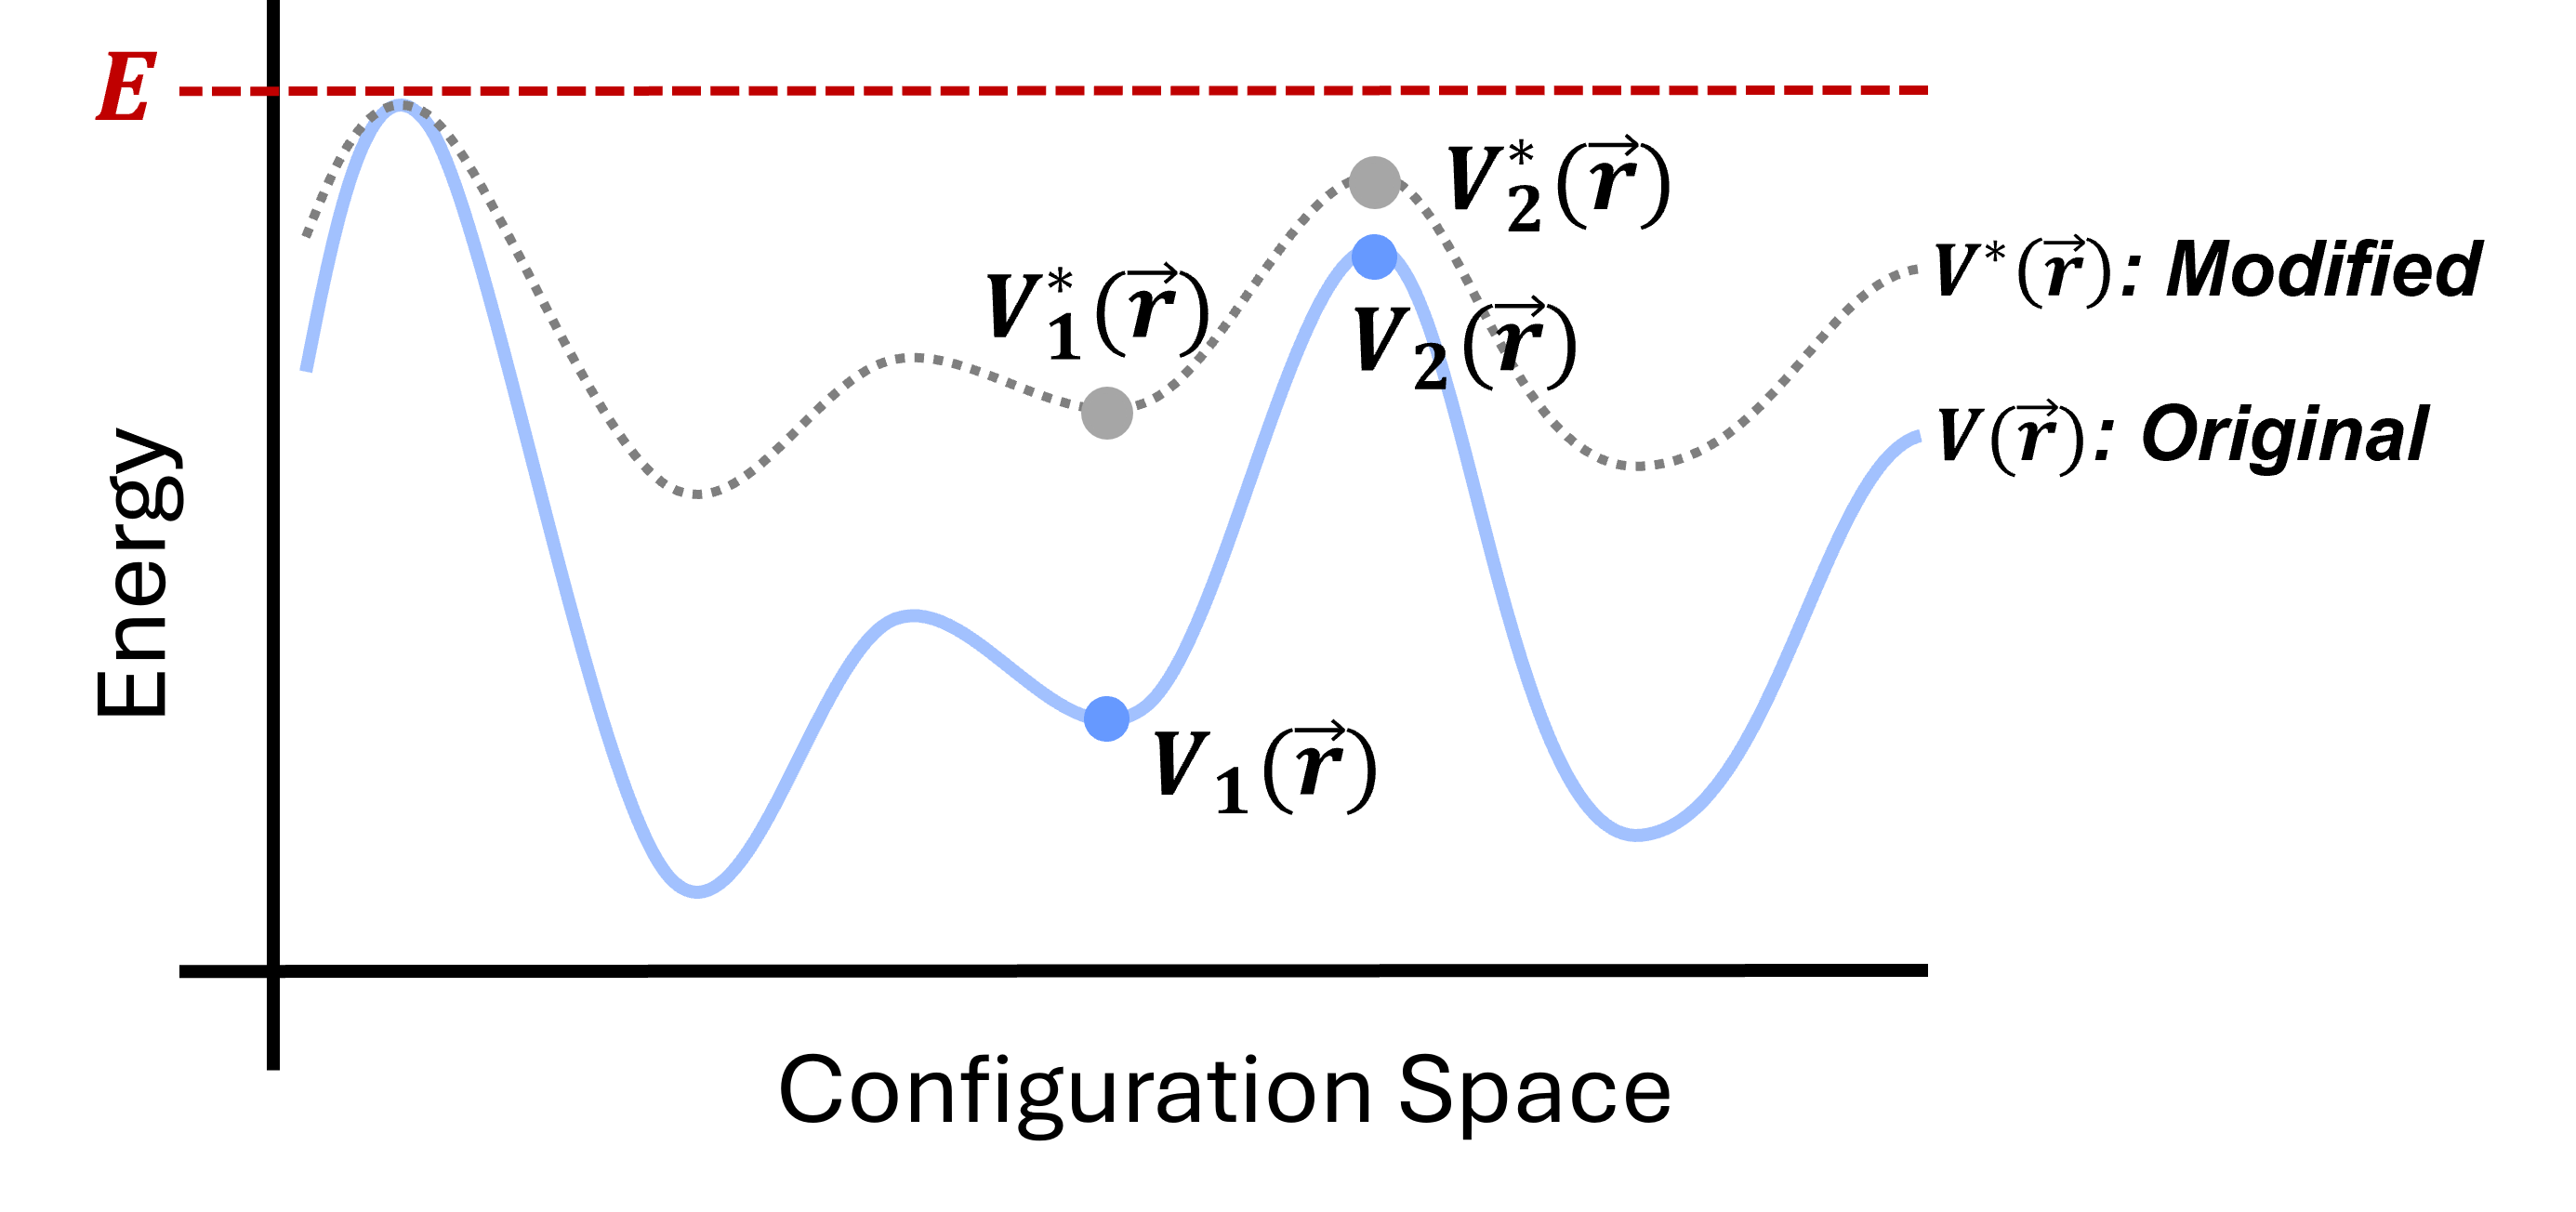
\includegraphics[width=\columnwidth]{main_figs/criteria1_2.png}
    \caption{Overview of the how boost potential criteria manifest in GaMD simulations. The original FES (light blue) is modified by boost potentials for any energy state below the threshold energy (red).}
    \label{fig:criteria12}
\end{figure}

If $V_{1}(\vec{r})$ < $V_{2}(\vec{r})$, then the respective potential energies on the boosted surface will also follow the same trend, $V_{1}^{*}(\vec{r})$ < $V_{2}^{*}(\vec{r})$, to maintain the shape of the original FES. 

\begin{equation*}
    \boxed{(1)\quad V_{1}\left(\vec{r}\right) < V_{2}\left(\vec{r}\right) \implies V_{1}^{*}\left(\vec{r}\right) < V_{2}^{*}\left(\vec{r}\right)}
\end{equation*}

In addition, the difference between the boosted energies should also be less than the difference of the original energies, $V_{1}^{*}\left(\vec{r}\right) - V_{2}^{*}\left(\vec{r}\right) < V_{1}\left(\vec{r}\right) - V_{2}\left(\vec{r}\right)$. This criterion ensures we are lowering the energy barriers.

\begin{equation*}
    \boxed{(2)\quad V_{1}\left(\vec{r}\right) < V_{2}\left(\vec{r}\right) \implies \left[V_{1}^{*}\left(\vec{r}\right) - V_{2}^{*}\left(\vec{r}\right)\right] < \left[V_{1}\left(\vec{r}\right) - V_{2}\left(\vec{r}\right)\right]}
\end{equation*}

If the first two criteria are combined in terms of $V^{*}(\vec{r})$, the value of $E$ must exist between $V_{max}$ and $V_{min} + \frac{1}{k}$, in which case $k \leq \frac{1}{V_{max} - V_{min}}$. If we define $k \equiv k_{0} \cdot \frac{1}{V_{max} - V_{min}}$, $k_{0}$ must be between 0 and 1. This requirement will be important for monitoring simulation convergence during GaMD equilibration and determines the extent to which conformational sampling is accelerated. 

Finally, the distribution of potential energies needs to be sufficiently narrow to allow the system to be properly reweighted. More details on reweighting will be provided in Section~\ref{ss:reweighting}). 

\begin{equation*}
    \boxed{
    \begin{gathered}
        (3)\quad\text{Narrow $\Delta{V}$ distribution} \\
        \sigma_{\Delta{V}} = k(E-V_{avg})\sigma_{V} \leq \sigma_{0} \\
        \text{where} \quad \sigma_{0}= k_{B}T
    \end{gathered}
    }
\end{equation*}

The value of $\sigma_{\Delta{V}}$ is the standard deviation of the boost potential, while $\sigma_{V}$ and $\sigma_{0}$ are the standard deviations of the potential energy in the current simulation step and the thermal energy, $k_BT$, at the simulation temperature, respectively. Enforcing $\sigma_{0} = k_BT$ ensures that the distribution of $\Delta{V}$ is within the desired statistical mechanical ensemble.

The potential energy standard deviation is used alongside $V_{max}$, $V_{min}$, and $V_{avg}$ to calculate $k_{0}$ in a manner that depends on whether $E$ is set to the ``lower bound'' $\left(E=V_{max}\right)$ or  ``upper bound'' $\left(E=V_{min}+\frac{1}{k}\right)$ condition. When $E$ is set to lower bound, $k_0$ is calculated according to Eq.~\ref{eqn:k0lower}:

\begin{equation}
    k_{0} = \text{min}\left(1.0,k_{0}^{'}\right) = \text{min} \left (1.0, \frac{\sigma_{0}}{\sigma_{V}} \cdot \frac{V_{max} - {V_{min}}}{V_{max} - V_{avg}} \right) 
    \label{eqn:k0lower}
\end{equation}

such that $k_{0}$ is set to 1 or $k_{0} = \frac{\sigma_{0}}{\sigma_{V}} \cdot \frac{V_{max} - {V_{min}}}{V_{max} - V_{avg}}$, whichever is lower. In the case of an upper bound condition, $k_{0}$ is calculated via Eq.~\ref{eqn:k0upper}:

\begin{equation}
    k_{0} = k_{0}^{''} \equiv \left (1.0 - \frac{\sigma_{0}}{\sigma_{V}} \right) \cdot \frac{V_{max} - {V_{min}}}{V_{avg} - V_{min}}
    \label{eqn:k0upper}
\end{equation}

only if $k_{0}^{''}$ is between 0 and 1. If $k_{0}^{''}$ is not between 0 and 1 then $k_{0}$ will be calculated via Eq.~\ref{eqn:k0lower}. $k_{0}$ can range from any value between 0 and 1, with higher $k_{0}$ values corresponding to larger boost potentials being added to the energy surface and thus greater acceleration of conformational sampling. $k_{0}$ is then used to calculate $k$ and ultimately used to determine the boost using Eq.~\ref{eqn:boost} and~\ref{eqn:deltav}.

\bigskip
\subsection{Reweighting}
\label{ss:reweighting}
Once GaMD simulations are complete, the modified energy surface is reweighted to recover the original energy surface. There are many different methods that can be used to reweight enhanced sampling simulations, but in the case of GaMD, it has been shown that cumulant expansion to the second order is the most efficient way to obtain the original FES as it was found to be less noisy than exponential reweighting and the use of Maclaurin series expansion~\cite{miao_improved_2014}. To perform reweighting, the PyReweighting toolkit of Python scripts has been developed for reweighting aMD and GaMD simulations using either the exponential average, Maclaurin series expansion, or cumulant expansion. In the case of GaMD, we are using cumulant expansion, an expansion of mathematical expressions to approximate a distribution of the boosts applied across the simulation time to determine the probability, and associated free energy, of each state in the system. 

GaMD simulations generate a biased probability distribution of states sampled in the trajectory. This biased distribution has energetic barriers that are generally lower than what would be found in the original distribution and are determined by the change in system potential energy or the boost, $\Delta{V(\vec{r})}$, applied at the specified frame in the simulation (Figure~\ref{fig:criteria12}). The amount of boost applied can then be converted to weights that relate the biased probability distribution to the original probability distribution over a specified CV used to describe transitions in the system. For large biomolecules (e.g., with millions of atoms), 0.5-1 million frames are suggested to ensure that there is enough boost data to accurately reweight, which corresponds to saving simulation frames every 0.1 ps~\cite{miao_gaussian_2015, pang_gaussian_2017, copeland_gaussian_2022}. This tutorial will not go over CV selection as this issue has been discussed elsewhere~\cite{bhakat_collective_2022}, however, it is essential that the CV best describes the system characteristics to answer the underlying research question.

Reweighting begins by reducing the dimensionality of the simulation data to correspond to the CV that is chosen to best describe the different states of a transition to be characterized. The range of possible CV values is divided into bins, or discrete intervals of the entire CV data range. As such, the simulation frames are sorted into these bins to determine how frequently different values of the CV are visited during the simulation. In each of these bins, the CV value and associated boost value are stored for that specific simulation frame. Since the GaMD algorithm is pushing the simulation to visit low-probability states, there needs to be a correction factor to offset the boost that was added. For each simulation frame, the boost is used to calculate this correction, which is then averaged across all bins to give an ensemble-averaged reweighting factor (This is shown in Eq.~\ref{eqn:reweightfactor}):

\bigskip
\bigskip

\begin{equation}
    \eqnmarkbox[Violet]{nume}{\left\langle e^{\beta\Delta{V\left(\vec{r}\right)}} \right\rangle} = \text{exp}
    \tikzmarknode{summ}{\left\{ \sum\limits_{k=1}^{\infty} \frac{\beta^{k}}{k!} C_{k} \right\}}
    \label{eqn:reweightfactor}
    \end{equation}
\annotate[yshift=1.2em, align=center, color=Black]{above,right}{nume}{Ensemble-Averaged \\ Reweighting Factor}


where $\beta$ = 1/$k_{B}T$ and the angle brackets, $\left\langle \right\rangle$, signify the averaging that occurs across the simulation ensemble. Essentially, the summation ($\sum$) can be expanded to however many mathematical terms the user deems necessary. Previous work has determined that using two ``cumulants'' (terms) was the most efficient method for GaMD reweighting~\cite{miao_improved_2014}. For example, the first three expanded terms that can be substituted for $C_{k}$ are shown in Eq.~\ref{eqn:cumulants}:

\bigskip

\begin{equation} 
    \begin{aligned}
    C_{1} & = \Delta{V}, & \text{``first order''} \\
    C_{2} & = \left\langle \Delta{V^{2}} \right\rangle - \left\langle \Delta{V^{2}} \right\rangle = \sigma_{v}^{2} & \text{``second order''} \\
    C_{3} & = \left\langle \Delta{V^{3}} \right\rangle - 3\left\langle \Delta{V^{2}} \right\rangle \left\langle \Delta{V} \right\rangle + 2\left\langle \Delta{V}^2 \right\rangle & \text{``third order''}    
    \end{aligned}
    \label{eqn:cumulants}
\end{equation}

\bigskip

Thus, if using cumulant expansion to the second order, the reweighting factor becomes equal to the summation of the series for cumulants 1 and 2 in Eq.~\ref{eqn:cumulants}. The reweighting factor is calculated for every frame in the simulation and determines how much that simulation frame should contribute to the original probability distribution. The biased probability distribution, $p^{*}(A_{j})$, is simply frequency of CV sampling without considering the boost potential. For each bin, $j$, the reweighting factors of all corresponding simulation frames are averaged to determine the ensemble-averaged reweighting factor. The ensemble-averaged reweighting factor is then multiplied by $p^{*}(A_{j})$ to rescale the distribution based on the magnitude of the boost potential in each bin. The result is then normalized by dividing by the total reweighting factor to obtain the original probability distribution, $p(A_{j})$, as shown in Eq.~\ref{eqn:probdist}: 

\bigskip
\bigskip
\bigskip

\begin{equation}
    \eqnmarkbox[Fuchsia]{origdist}{p\left(A_{j}\right)} =
    \eqnmarkbox[Thistle]{biasdist}{p^{*}\left(A_{j}\right)} 
    \frac{ 
    \eqnmarkbox[Violet]{nume}{\left\langle e^{\beta\Delta{V\left(\vec{r}\right)}} \right\rangle}_{j}}
    {\eqnmarkbox[CadetBlue]{denom}{\sum_{j=1}^{M} \left\langle p^{*}\left(A_{j}\right)e^{\beta\Delta{V\left(\vec{r}\right)}} \right\rangle_j}
    }, \quad
    \eqnmarkbox[OliveGreen]{bin}{j=1, ..., M}
    \label{eqn:probdist}
\end{equation}
\annotate[yshift=1.2em, align=center, color=Black]{above,right}{origdist}{Original Probability \\ Distribution}
\annotate[yshift=-0.5em, align=center, color=Black]{below,left}{biasdist}{Biased Probability \\ Distribution}
\annotate[yshift=1.2em, align=center, color=Black]{above,right}{nume}{Ensemble-Averaged \\ Reweighting Factor}
\annotate[yshift=-1em, align=center, color=Black]{below}{denom}{Total Boltzmann Reweighting \\ Factor Across All Bins}
\annotate[yshift=0.75em, align=center, color=Black]{right}{bin}{Bin Number}

\bigskip
\bigskip
\bigskip
\bigskip

Doing so redistributes the probability density based on the GaMD boost, correcting for over-sampling of high energy states and under-sampling of low-energy states. In addition to the probability distribution, the free energy is also calculated using cumulant expansion to the second order shown in Eq.~\ref{eqn:reweightfreener1}:

\bigskip
\bigskip

\begin{equation} 
    \eqnmarkbox[PineGreen]{reweight_fe}{F\left(A_{j}\right)} = \eqnmarkbox[Green]{mod_fe}{F^{*}\left(A_{j}\right)} - \sum\limits_{k=1}^{2}\frac{\beta^{k}}{k!} C_{k} + 
    \eqnmarkbox[YellowGreen]{force}{F_{c}}
    \label{eqn:reweightfreener1}
\end{equation}
\annotate[yshift=1.2em, align=center, color=Black]{above,left}{reweight_fe}{Reweighted \\ Free Energy}
\annotate[yshift=1.2em, align=center, color=Black]{above,right}{mod_fe}{Biased \\ Free Energy}
\annotate[yshift=1.2em, align=center, color=Black]{above,right}{force}{Force Constant}


Finally, the reweighted energy profile for each bin, $j$, can be calculated using the reweighted free energy, $F(A_{j})$, and the original probability distribution, $p(A_{j})$, using Eq.~\ref{eqn:reweightfreeener2}:

\bigskip
\bigskip
\bigskip

\begin{equation}
    \eqnmarkbox[PineGreen]{reweight_fe}{F\left(A_{j}\right)} = -\frac{1}{\beta} ln
    \eqnmarkbox[Fuchsia]{origdist}{p\left(A_{j}\right)}
    \label{eqn:reweightfreeener2}
\end{equation}
\annotate[yshift=1.2em, align=center, color=Black]{above,left}{reweight_fe}{Reweighted \\ Free Energy}
\annotate[yshift=1.2em, align=center, color=Black]{above,right}{origdist}{Original Probability \\ Distribution}

The reweighted free energy and the associated CV values can then be plotted and used to evaluate the FES.                                                                                                 

\begin{figure*}[ht!]
    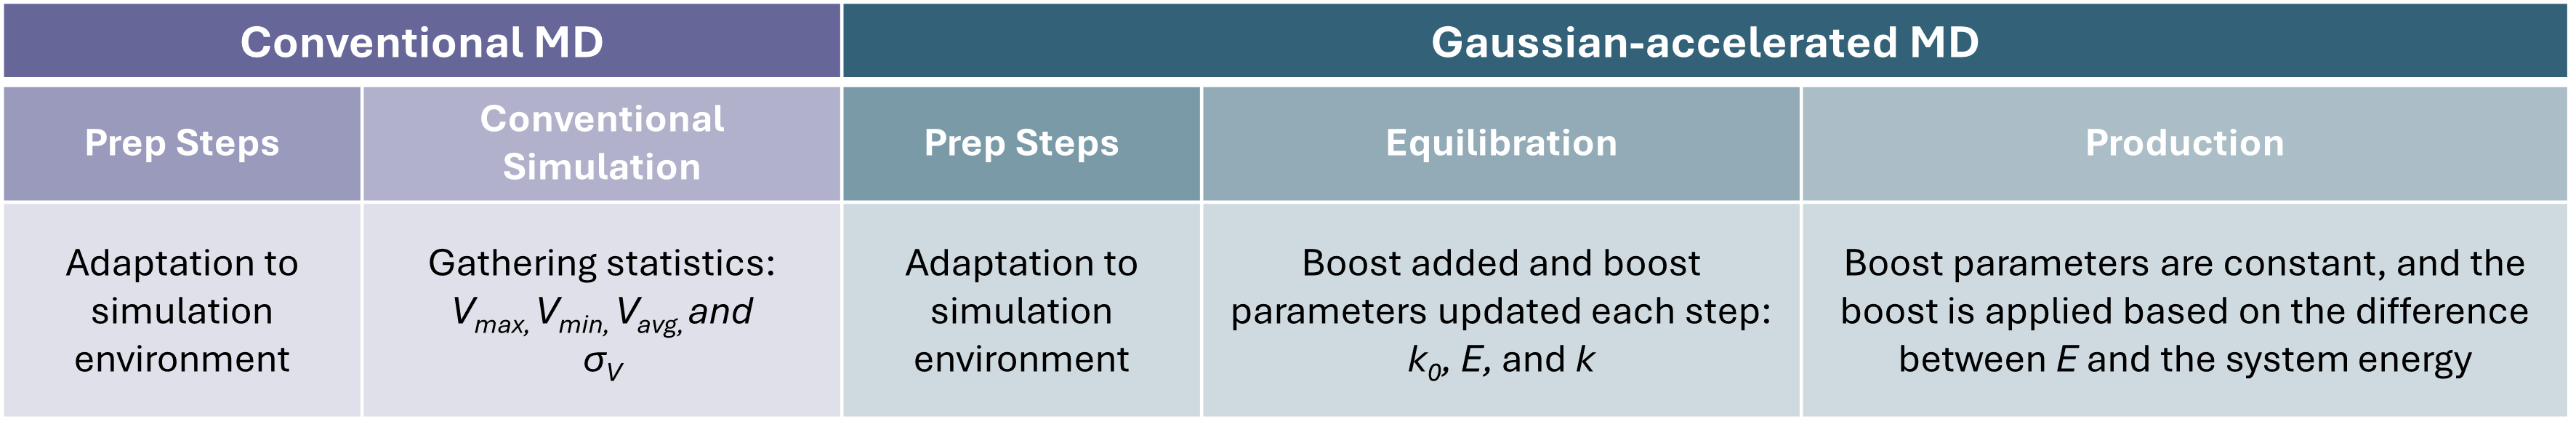
\includegraphics[scale=0.68]{main_figs/gamd_overview.png}
    \caption{Overview of the GaMD process in NAMD.}
    \label{fig:gamdoverview}
\end{figure*}



\section{Workflow of Running a GaMD Simulation} \label{sec:workflow}
The GaMD procedure in the NAMD suite consists of three distinct stages. First, a short conventional MD simulation gathers initial energetic information and calculates thermodynamic statistics of the system such as $V_{max}$, $V_{min}$, $V_{avg}$, and $\sigma_{V}$. Then, an equilibration step is used to update these statistics and refine the harmonic force constant, $k$ using Eqs.~\ref{eqn:k0lower} and~\ref{eqn:k0upper}; the threshold energy, $E$ using Eq.~\ref{eqn:threshold}; and the boost potential using Eq.~\ref{eqn:boost}. Finally, a GaMD production simulation of user-defined length is performed using the established threshold energy from equilibration and boosts are applied to enhance the conformational sampling. A simplified overview of these steps and their general function is given in Figure~\ref{fig:gamdoverview}.

\subsection{Overview of the Run Scripts}
As mentioned previously, we will focus on how to specify a GaMD simulation within a NAMD run script. Templates for the inputs can be found on the Miao lab website ( ~\url{https://www.med.unc.edu/pharm/miaolab/resources/gamd/tutorial-of-gamd-in-namd/}) and our full scripts can be found in the GitHub repository accompanying this article (\githubrepository). In general, the GaMD section has the following form:

\begin{lstlisting}[label=run_script,caption=Conventional and Equilibration Setup, basicstyle=\small, backgroundcolor=\color{light-gray}]
#########################################
## GAMD                    
#########################################
accelMD                  <on/off>	           
accelMDdual              <on/off>	           
accelMDdihe              <on/off>               
accelMDG                 <on/off>	           
accelMDGiE               <1/2>                               
accelMDGcMDPrepSteps     <number of steps>      
accelMDGcMDSteps         <number of steps>	   
accelMDGEquiPrepSteps    <number of steps>      
accelMDGEquiSteps        <number of steps>      
accelMDOutFreq           <number of steps>      

accelMDGStatWindow       <number of steps>	   

accelMDGsigma0P          <value>		             
accelMDGsigma0D          <value>

accelMDGRestart          <on/off> 
accelMDGRestartFile      <file name> 

\end{lstlisting}

\bigskip
A full description of all GaMD parameters and their default values for NAMD can be found in the NAMD manual (\url{https://www.ks.uiuc.edu/Research/namd/2.14/ug/node70.html}). Here we will provide a synopsis of each term:

\bigskip

\begin{description}
    \item[accelMD] Specifies whether accelerated MD is to be turned on or off. GaMD is an extension of aMD, so this setting must be on if you are using GaMD.
    \item[accelMDdual] Specifies whether to apply ``dual-boost'' GaMD.
    \item[accelMDdihe] Specifies whether to apply dihedral boost. If ``dual-boost'' is on, then this keyword must be set to ``on'' as well. Doing so will provide the greatest sampling acceleration.
    \item[accelMDG] Specifies the use of GaMD as the accelerated MD method.
    \item[accelMDGiE] Sets $E$ to either the lower bound (1) or upper bound (2). Lower bound (1) sets $E$ to $V_{max}$ and is the typical setting.
    \item[accelMDGcMDPrepSteps] Number of preparatory conventional MD steps.
    \item[accelMDGcMDSteps] Number of conventional MD steps after preparatory steps.
    \item[accelMDGEquiPrepSteps] Number of preparatory GaMD equilibration steps.
    \item[accelMDGEquiSteps]  Number of GaMD equilibration steps after preparatory steps.
    \item[accelMDOutFreq] Specifies the output frequency of the GaMD algorithm.
    \item[accelMDGStatWindow]  Sets how often to calculate the average and standard deviation of the boost potential during GaMD. This value should be set to $\sim4\times$ the number of particles in the simulation system.
    \item[accelMDGsigma0P] Upper limit of the standard deviation of the total boost potential.
    \item[accelMDGsigma0D] Upper limit of the standard deviation of the dihedral boost potential.
    \item[accelMDGRestart] Specifies whether or not this simulation is being restarted from a previous one. Ensures that the \texttt{*.gamd} file is read to restart. 
    \item[accelMDGRestartFile] Specifies the name of the GaMD restart file.
\end{description}

\bigskip

\subsection{Running Conventional Simulations and GaMD Equilibration} \label{ss:cmd_gamd_equil}
Initially, GaMD starts with a specified number of conventional simulation steps during which no boost is applied to the system. This step gathers statistics related to the potential energy of the system, including $V_{max}$, $V_{min}$, $V_{avg}$, $\sigma_{V}$, $E$, $k_{0}$, and $k$. To start the simulations, NAMD will require information about the structure of interest and the topology. Using this starting information, a short segment of preparatory steps (\texttt{accelMDGcMDPrepSteps}) is conducted before the conventional simulation segment to allow the biomolecule to adapt to its simulation environment, basically to ensure the simulation will not crash. The user can specify any amount of steps for these different segments. Generally, the preparatory steps require less simulation time and therefore fewer steps since they are not used to collect statistics and refine the boost potential. This tutorial will not recommend a specific number of steps for each segment but previous studies using GaMD have employed 200,000 steps for the preparatory segment and 200,000 steps for the conventional segment when simulating larger biomolecules. Our chosen number of steps for alanine dipeptide will be discussed in Section~\ref{sec:tutorial}.

Once the conventional segment is complete, equilibration preparatory steps will be conducted, followed by the equilibration segment. During the equilibration segment, the statistics are refined and $E$ is allowed to increase until it levels off. Boosts are also applied during this stage and refined based on the changes to $E$. Prior work states that $k_{0}$ should stabilize or reach 1 throughout equilibration to determine if your equilibration simulation has reached convergence~\cite{miao_gaussian_2015}. However, we have found that it may also be beneficial to track $V_{max}$, as it still can increase even when $k_{0}$ reaches 1. We will discuss more on interpreting the output files in and monitoring the simulations in Section~\ref{ss:interpret_output}. If equilibration does not reach convergence in the designated number of steps, it can be extended using the GaMD restart file and by setting \texttt{accelMDGcMDPrepSteps}, \texttt{accelMDGcMDSteps}, and \texttt{accelMDGEquiPrepSteps} to \texttt{0}. Both conventional MD and GaMD equilibration are executed from the same script, which we have named \texttt{gamd\_equil.in} and can be found in each force field directory in the GitHub repository.

\subsection{Running GaMD Production}
\label{ss:gamd_production}
Once it has been established that the GaMD equilibration has converged by monitoring $k_{0}$ and $V_{max}$, the system can proceed to the production stage. At the end of equilibration, the value of $E$ is set and does not change throughout production. Here, boosts are applied based on the difference between $E$ and the potential energy at the current step in the simulation, $V\left(\vec{r}\right)$. The larger the difference in $E$ and $V\left(\vec{r}\right)$, the larger the magnitude of boost applied. 

The run script is generally the same as the one used for conventional and equilibration, however, no conventional or equilibration steps will be performed. As such, \texttt{accelMDGcMDPrepSteps}, \texttt{accelMDGcMDSteps}, \texttt{accelMDGEquiPrepSteps}, and \texttt{accelMDGEquiSteps} are all set to \texttt{0}. The \texttt{run} parameter can be adjusted, as well, to suit a user's specific needs in terms of production simulation length. In addition, \texttt{accelMDGRestart} will need to be set to ``on'' so that the GaMD statistics and $E$ can be read in from the restart file, \texttt{gamd\_equil.gamd}. An example of the GaMD parameters for production is as follows:

\begin{lstlisting}[label=gamd_prod,caption=md.*.in, basicstyle=\small,backgroundcolor=\color{light-gray}]
#########################################
## GAMD                    
#########################################
accelMD                  on             
accelMDdual              on
accelMDdihe              on
accelMDG                 on        
accelMDGiE               1             
         
accelMDGcMDSteps         0        
accelMDGEquiSteps        0     
accelMDGcMDPrepSteps     0         
accelMDGEquiPrepSteps    0         
accelMDOutFreq           500

accelMDGStatWindow       10000

accelMDGsigma0P          6.0            
accelMDGsigma0D          6.0 

accelMDGRestart          on 
accelMDGRestartFile      <BASENAME>.gamd  

\end{lstlisting}

In principle, the GaMD production can be performed for any length of time, but for practicality, we suggest running the GaMD production simulations in strides. This way, trajectories and all output files are saved in increments and in the case of crashes or file corruption, only short intervals of data are lost rather than the entire simulation. Generally, the production input files will look the same but variables are read in from a separate bash script to automate the setup of short strides. We will overview how we generate the strides in more detail in Section~\ref{ss:tutorial_prod}. Both the submission script and the template script can be found on GitHub and are named \texttt{sub\_gamd\_prod.sh} and \texttt{md.template}.

\subsection{Interpreting GaMD Output Files}
\label{ss:interpret_output}
Throughout the GaMD process, several output files are created to monitor progress and continue running the simulation. Many of these files are generated by NAMD, and not the GaMD algorithm itself, including:

\begin{itemize}
    \item \texttt{.coor} - PDB-formatted atomic coordinates.
    \item \texttt{.xsc} - the extended system restart information.
    \item \texttt{.vel} - PDB-formatted atomic velocities.
    \item \texttt{.xst} - all the extended system information over time. 
    
\end{itemize}

The GaMD algorithm produces two files: the log file, \texttt{gamd\_equil.out} or \texttt{md.*.out}, that contains all the thermodynamics statistics of your system throughout the GaMD process; and the GaMD restart file, \texttt{gamd\_equil.gamd} or \texttt{*.gamd}, that contains information about the current stage of GaMD and is required to continue running a simulation from where it left off. GaMD equilibration will create one of each of these files, whereas every stride during production will have its own set of these output files.

Taking a closer look at \texttt{gamd\_equil.out} in Listing~\ref{log}, this file contains the step by step output of GaMD and is a critical output file to inspect. All of the statistical data collected by the GaMD algorithm for each simulation step is found within this file. The top portion of this file details the NAMD environment setup for the simulation. The simulation has started running when the \texttt{run} keyword is executed and the number of steps for the simulation is printed to the \texttt{.log} files (Listing~\ref{log}, first line). Below this line, the GaMD algorithm will start printing the system potential energy statistics to the output file. These lines are used to track the statistics over time, verify that each stage is running correctly, and to monitor statistics throughout the simulation. An example of this section at the start of the conventional preparatory steps is shown in Listing~\ref{log}.

\begin{figure*}[h!]
\begin{lstlisting}[label=log,caption=gamd\_equil.out, basicstyle=\small,breaklines=true, backgroundcolor=\color{light-gray}]
TCL: Running for 26100000 steps

""

ACCELERATED MD: STEP 0 dV 0 dVAVG 0 BOND 0.000398329 ANGLE 0.758706 DIHED 4.07314 IMPRP 0.074434 ELECT -9757.12 VDW 1176.49 POTENTIAL -8575.72
GAUSSIAN ACCELERATED MD: DIHED iE 1 Vmax 4.07314 Vmin 4.07314 Vavg 4.07314 sigmaV 0 E 0 k0 0 k 0
GAUSSIAN ACCELERATED MD: TOTAL iE 1 Vmax -8579.8 Vmin -8579.8 Vavg -8579.8 sigmaV 0 E 0 k0 0 k 0
   
\end{lstlisting}
\end{figure*}

The aMD and GaMD algorithms report on the state of the system at the current step. The example shown in Listing~\ref{log} represents step 0, or the initial state of the system in the current GaMD run. On the \texttt{ACCELERATED MD} line, \texttt{dV} is the boost at the current step, which, for dual-boost, is actually the sum of the dihedral and total potential boosts as described in Eq~\ref{eqn:sumboost}: 

\bigskip

\begin{equation}
    \eqnmarkbox{sumdV}{\Delta{V}} =
    \eqnmarkbox[Peach]{dVT}{\Delta{V_{T}}}+
    \eqnmarkbox[Apricot]{dVD}{\Delta{V_{D}}}
    \label{eqn:sumboost}
\end{equation}
\annotate[yshift=1em, align=center, color=Black]{right}{sumdV}{Overall Boost}
\annotate[yshift=-0.5em, align=center, color=Black]{below, left}{dVT}{Total Potential Boost}
\annotate[yshift=-0.5em, align=center, color=Black]{below, right}{dVD}{Dihedral Boost}

\bigskip

$\Delta{V_{T}}$ and $\Delta{V_{D}}$ are calculated using Eqn.~\ref{eqn:boost} and the energy values corresponding to the total potential energy, $V\left(\vec{r}\right)$, and the dihedral energy term, $V_{\tau}$.

\bigskip
\bigskip

\begin{equation} 
    \eqnmarkbox[Peach]{}{\Delta{V_{T}}} =\frac{1}{2}k \left\{
    \eqnmarkbox[Sepia]{thresh}{E_{T}} - \left[
    \eqnmarkbox[RoyalPurple]{currentnrg}{V\left(\vec{r}\right)} - 
    \eqnmarkbox[Plum]{dihenrg}{V_{\tau})}\right]\right\}^{2}
    \label{eqn:totboost}
\end{equation}
\annotate[yshift=1em, align=center, color=Black]{right}{currentnrg}{Current System \\ Potential Energy}
\annotate[yshift=1em, align=center, color=Black]{left}{thresh}{Threshold Energy}
\annotate[yshift=-0.5em, align=center, color=Black]{below, left}{dihenrg}{Dihedral Energy}

\bigskip

\begin{equation} 
    \eqnmarkbox[Apricot]{}{\Delta{V_{D}}} =\frac{1}{2}k \left\{
    \eqnmarkbox[Sepia]{}{E_{D}} - 
    \eqnmarkbox[Plum]{}{V_{\tau}}\right\}^{2}
    \label{eqn:totboost}
\end{equation}

\bigskip

On the same line \texttt{dVAVG} is the average boost up to the current point in the simulation. The remainder of this line reports the contributions of the various terms in the potential energy equation. For ``dual-boost'' GaMD, separate lines are printed to track statistics for the dihedral energy, \texttt{GAUSSIAN ACCELERATED MD: DIHED}, and the total potential energy, \texttt{GAUSSIAN ACCELERATED MD: TOTAL}. In these lines, \texttt{iE} indicates the setting of the threshold energy, and the remainder of the printed fields are the maximum, minimum, and average energy, the variation in energy, the threshold energy, \texttt{k0}, and the harmonic force constant for the current step. 

During conventional and equilibration preparatory steps, no potential energy statistics are updated, and as such \texttt{sigmaV}, \texttt{E}, \texttt{k0}, and \texttt{k} all remain \texttt{0}. Without statistics, no boost can be calculated so \texttt{dV} and \texttt{dVAVG} also remain \texttt{0} throughout the preparatory step segments. The statistics start to be reported during the conventional segment while the boost values remain zero until the equilibration stage. During equilibration, $E$ and the boost are updated in their respective field as the system explores the conformational landscape. Once equilibration convergence has been observed through monitoring of $k$ and $E$ (see Section~\ref{sec:tutorial}), $E$ is held constant for production, remaining consistent in the output files, and the boost is calculated each step using Eq.~\ref{eqn:boost}. 

Another output file, \texttt{*.gamd}, contains all the GaMD information from the last complete step. An example is shown in Listing~\ref{energyfile}. In it are two lines of information for the dihedral and total energies indicated by the single letter codes in the first column of the row, \texttt{D} and \texttt{T}. Following are the current step, \texttt{Vn}; the maximum energy, \texttt{Vmax}; the minimum energy, \texttt{Vmin}; the average energy, \texttt{Vavg}; the standard deviation, \texttt{sigmaV}; the variability from the mean, \texttt{M2}; the threshold energy, \texttt{E}; and \texttt{k}. For equilibration, only one \texttt{gamd\_equil.gamd} is produced, compared to production, during which a file is produced for each stride in our approach. 

\begin{figure*}
\begin{lstlisting}[label=energyfile,caption=system.gamd, basicstyle=\small,breaklines=true, backgroundcolor=\color{light-gray}]
# NAMD accelMDG restart file
# D/T Vn Vmax Vmin Vavg sigmaV M2 E k
D 10000 23.42610900347244 2.4217065108565792 8.5355531287135644 2.4186399083415688 5.84981900622251123e+04 23.42610900347244 0.04760906673501196
T 10000 -8188.84384705514 -9062.2482195580287 -8296.0966588262636 20.988071042745403 4.40499126095328107e+06 -8188.84384705514 0.00114494503517807             
\end{lstlisting}
\end{figure*}

\subsection{Reweighting}
\label{ss:reweight}
As mentioned previously, the PyReweighting toolkit can be found at \url{https://github.com/MiaoLab20/pyreweighting}. The PyReweighting toolkit allows for one-, two-, or three-dimensional reweighting, depending on how many CVs are chosen for this analysis. Within the \texttt{pyreweighting} directory, these options are represented by scripts named \texttt{PyReweighting-1D.py}, \texttt{PyReweighting-2D.py}, and \texttt{PyReweighting-3D.py}. Each of these scripts is executed by \texttt{reweight-1D.sh}, \texttt{reweight-2D.sh}, and \texttt{reweight-3D.sh}, respectively. The execution scripts determine what reweighting scheme will be used. In the \texttt{reweight-*.sh} scripts, there are four sections of code representing the types of reweighting schemes: cumulant expansion (\texttt{amdweight\_CE}), no weight (\texttt{noweight}), weight (\texttt{amdweight}), histogram (\texttt{histo}), and the boost potential (\texttt{amd\_dV}). As noted above, previous studies concluded that it is best to use cumulant expansion to the second order to reweight GaMD simulations~\cite{shen_statistical_2008, miao_improved_2014}, which is carried out using the (\texttt{amdweight\_CE}) argument. In addition to reweighting, it is also important to assess the anharmocity of the system to determine if the boosts applied follow a Gaussian distribution. The anharmonicity calculations are performed using the \texttt{amd\_dV} argument. All commands are already present in the \texttt{reweight-2D.sh} and an example is shown in Listing~\ref{reweight_script}.

\begin{figure*}[hbt]
\begin{lstlisting}[label=reweight_script,caption=reweight-2D.sh, basicstyle=\small,breaklines=true, backgroundcolor=\color{light-gray}]
python $dir_codes/PyReweighting-2D.py -input $data -T $T -Emax $Emax -cutoff $cutoff -discX $binx -discY $biny -job amdweight_CE -weight weights.dat | tee -a reweight_variable.log
\end{lstlisting}
\end{figure*}

The Python interpreter is used to execute the reweighting algorithm in \texttt{PyReweighting-2D.py}, which we use as an example in the tutorial that follows. All command-line arguments denoted with \texttt{\$} are variables that are specified in the \texttt{reweight-2D.sh} shell script. A complete list of the arguments present in this example as well as any additional arguments that may be beneficial in obtaining the most descriptive set of potential of mean force values for the chosen CVs are outlined below.

\begin{description}
    \item[input] (required) The file containing the chosen CVs, separated by column
    \item[job] (required) Choice of reweighting method
    \item[weight] (required) The file containing the weights from GaMD
    \item[Xdim] (optional) Specify dimensions for the first CV (x-axis)
    \item[Ydim] (optional) Specify dimensions for the second CV (y-axis)
    \item[discX] (optional) Discretion size (bin width) of first CV
    \item[discY] (optional) Discretion size (bin width) of second CV
    \item[cutoff] (optional) Minimum number of simulation frames required per bin
    \item[T] (optional) Temperature
    \item[Emax] (optional) Maximum free energy
    \item[fit] (optional) Fit $\Delta{V}$ distribution
    \item[order] (optional) Order of Maclaurin series to use in reweighting. May only be needed if not using cumulant expansion to the second order.
\end{description}

Each of the optional arguments is dependent on the system and is employed at the discretion of the user. In the alanine dipeptide tutorial that follows, we chose to add in \texttt{Xdim} and \texttt{Ydim}, which are set to the possible dimensions of $\phi$ and $\psi$ angles of the alanine dipeptide backbone.

The \texttt{-job} argument determines the type of reweighting and ultimately what output files are obtained. Setting \texttt{-job amdweight\_CE} provides the user with the potential of mean force (PMF) values for c1, c2, c3 using Eq.~\ref{eqn:cumulants}. Each file name contains the name of the data file used and the bin width specified, making it easier to track the parameters specified. For example, the file name \texttt{pmf-2D-c2-cv\_500.dat-reweight-discx15-discy15.xvg} indicates this file contains the energy values (\texttt{pmf}), from 2D reweighting performed using cumulant expansion to the second order (\texttt{c2}) across the CVs contained within \texttt{cv\_500.dat} with a bin width for x and y of 15 (\texttt{discx15} and \texttt{discy15}). Files beginning with \texttt{pmf-2D-c2} will be the primary files for GaMD reweighting. The file is organized with the first CV, x, and the second CV, y, in the first and second columns, followed by the PMF in the third column. This file will be used to generate the FES.

An additional quantity, ''anharmonicity'' or $\gamma$, can be used to characterize the distribution of the applied boosts. When $\gamma$ is zero, the boost is considered harmonic (\textit{i.e.} it follows a Gaussian distribution) and confirms that the reweighted free energy profiles are accurate. As $\gamma$ increases, $\Delta{V(\vec{r})}$ becomes less harmonic and indicates that the reweighted free energy profile deviates from the original energy profile. This value can help evaluate the quality of the FES and we will discuss this value in context in Section~\ref{ss:tutorial_reweight}.

\section{Tutorial} 
\label{sec:tutorial}
We will demonstrate the GaMD protocol with a small system of the alanine dipeptide in water. To illustrate several important principles and outcomes, we will compare results of this protocol that arise from using the AMBER ff19SB~\cite{tian_ff19sb_2020}, CHARMM36m~\cite{huang_charmm36m_2017}, and Drude-2019~\cite{lin_further_2020} force fields. 

\subsection{Introduction}
Alanine dipeptide has long been used as a model system for validating force field parameters and simulation methods, and has been used as the published test system for GaMD~\cite{miao_gaussian_2015, pang_gaussian_2017, copeland_gaussian_2022}. This tutorial will focus on instructing users on how to set up, reweight, and analyze alanine dipeptide GaMD simulations, with a comparison among the results of the three different force fields. The reweighting process using the PyReweighting toolkit will also be demonstrated along with a discussion on how to adjust specific GaMD parameters for the system of interest. The GitHub repository associated with this article (\githubrepository) contains all scripts and input files required to complete the tutorial.

\subsection{GaMD System Preparation} 

\subsubsection{The System}
We are interested in the conformational sampling of alanine dipeptide. Three systems were prepared using the AMBER ff19SB, CHARMM36m, and Drude-2019 force fields which we will refer to as ff19SB, C36m, and Drude, respectively. Details on how to construct each system with their respective FF will not be given here, and the user should construct and minimize their system in whatever manner is appropriate. Briefly, the AMBER ff19SB system was constructed using AmberTools~\cite{case_ambertools_2023} and then converted to C36m. The Drude system was then constructed from the C36m system using the CHARMM program~\cite{hwang_charmm_2024}. Initial C36m and Drude structures were obtained from a brief minimization using a previously published protocol~\cite{lemkul_preparing_2021}.

\subsubsection{Setting Up the Working Directories} 
Topology and coordinate files for each system are located in the directory named according to the force field used (\texttt{ff19sb}, \texttt{c36}, and \texttt{drude} in our case). For AMBER ff19SB, the parameter and topology file (\texttt{ala.parm7}) and the coordinate file (\texttt{ala.rst7}) should be placed within the \texttt{ff19sb} directory while for C36m and Drude, \texttt{ala.c36.psf} and \texttt{ala.c36.pdb} should be placed in \texttt{c36m} and \texttt{ala.drude.psf} and \texttt{ala.drude.pdb} should be placed in \texttt{drude}. A directory for GaMD equilibration and production should be created in the directory corresponding to each system. For clarity, we named these directories \texttt{equil} and \texttt{prod}. Dynamics input files for equilibration, (\texttt{gamd\_equil.in}) and production (\texttt{md.template}), and submission scripts for SLURM queueing (\texttt{sub\_gamd\_equil.sh} and \texttt{sub\_gamd\_prod.sh}) can be found in the associated force field directories on GitHub and should also be placed in the respective equilibration and production directories. All force field parameters for ff19SB are found within the parm7 file while the parameter files for C36m and Drude systems are listed in the run scripts and can be obtained from the MacKerell lab website (\url{https://mackerell.umaryland.edu/charmm_drude_ff.shtml}), if required. 

\subsection{Contents of the Run Scripts and Parameters for Equilibration} 
We have provided complete run scripts for conventional MD/GaMD equilibration and GaMD production for each force field as they each require distinct NAMD keywords. We encourage users to ensure that they have the correct script for the force field applied to the system. In general, the scripts provided will need minimal adjusting to reflect system input files, designated force field, system properties, and the length of time for each of the GaMD steps. The preparatory, conventional MD, and GaMD equilibration steps will all be initialized from the \texttt{gamd\_equil.in} input script, while the production step will be run in short intervals (or ``strides'') from a template script, which will be described in more detail in Section~\ref{ss:tutorial_prod}. As a general suggestion,users should review all scripts for any NAMD parameters that need to be adjusted for their specific system prior to running the actual simulations. The input files for this tutorial should only require adjustment on specifying locations of force field files. Here, we will provide an overview of the sections of the NAMD input files and provide information regarding the NAMD parameters or keywords that we will use for alanine dipeptide. This first section will focus on NAMD keyword selections for conventional MD and GaMD equilibration, while the information for GaMD production will be provided in Section~\ref{ss:tutorial_equil}. 

\subsubsection{Coordinate, Topology, Force Field and Other Input Files}
This section specifies the input topology and coordinate files. C36m and Drude use NAMD keywords \texttt{coordinates} and \texttt{structure} for the PDB and PSF files respectively, while ff19SB systems are specified with NAMD keywords \texttt{ambercoor} and \texttt{parmfile} for the rst and parm7 files. In the associated script, we have specified the force field parameter files using \texttt{parameters} for C36m and Drude. NAMD also requires the format of the force field parameters to be stated through keywords \texttt{amber} for ff19SB and \texttt{paraTypeCharmm} for C36m and Drude. There are several other keywords in this section that can be adjusted depending on what system is running; \texttt{mergeCrossterms} for C36m, Drude, and ff19SB, and \texttt{readexclusions} and \texttt{scnb} for ff19SB. The details of each of these keywords can be found in the NAMD manual. Temperature (K) and time step (in femtoseconds, fs) are also set in this section using the \texttt{temperature} and \texttt{timestep} keywords. These settings generally depend on the system of interest but for alanine dipeptide we will simulate at 298 K and use a timestep of 2.0 fs for ff19SB and C36m and a timestep of 1.0 fs for Drude. 

\subsubsection{Output Files and Output Frequency}
The output section specifies what type of output files are desired as well as what to name them. We set NAMD keywords \texttt{outputname}, \texttt{dcdfile}, and \texttt{restartname} such that all outputs will have the prefix \texttt{gamd\_equil} for the GaMD equilibration stage. 

Output parameters specify how often the respective properties are written to output files. The user indicates a number of steps for these keywords, which can then be multiplied by the time step to determine how often the output files are updated. As mentioned previously, saving $0.5 - 1 \times 10^6$ frames is recommended to ensure there is enough simulation data to accurately reweight. Since alanine dipeptide is a small system, we have set our scripts to update the output every 1 ps (500 steps for systems with 2 fs timestep, and 1000 steps for systems with 1 fs time step). 

\subsubsection{Temperature and Pressure Control}
This section details the type of thermostat and barostat to use for the simulations. For all systems, we specify the use of Langevin dynamics (\texttt{Langevin}) via the Langevin thermostat and barostat~\cite{feller_langevinpiston_1995} (\texttt{LangevinPiston}), and the temperature at which the system is maintained (\texttt{LangevinTemp}).

\subsubsection{Non-bonded Setup}
This section contains information on how each system handles non-bonded interactions. The \texttt{switching} keyword will turn on the switching function for C36m and Drude and \texttt{vdwForceSwitching} should be specified for C36m only. Other parameters will depend on the force field used. The short-range non-bonded cutoff, switching function distance, exclusions, neighbor searching radius, 1-4 interaction scaling, and dielectric can all be set in this section. This section also contains optional keywords to specify a Drude system, with keyword \texttt{drude}, and other Drude-specific settings to turn on or off the hard wall constraint, specify the Drude-atom bond distance at which the hard wall acts, set the through-space Thole cutoff, etc. 

\subsubsection{Constraints}
This section contains keywords for bond constraints. \texttt{rigidbonds} determines what, if any, atoms are constrained. For these systems, all the bonds connecting hydrogens to their parent atoms are constrained and so are all water molecules. \texttt{rigidTolerance}, \texttt{rigidIterations}, and \texttt{useSettle} determine the maximum bond-length error, the number of attempts to constrain bond lengths, and employ the SETTLE algorithm to water molecules.

\subsubsection{Electrostatics}
This section details the settings related to the use of the particle mesh Ewald algorithm for electrostatics~\cite{darden_pme_1993}. Here, the use of  \texttt{PME} is specified along with the number of Fourier lattice grid points in each direction using \texttt{PMEGridSizeX}, \texttt{PMEGridSizeY}, and \texttt{PMEGridSizeZ}.

\subsubsection{Unit Cell Definition}
This section details the size of the simulation box and the cell origin. \texttt{wrapAll} indicates whether or not periodic boundary conditions should be active for all atoms and is typically used for simulations during which no restraints are applied. 

\subsubsection{GaMD Settings}
This section contains the GaMD-specific settings previously described in Section~\ref{sec:workflow}. Here, \texttt{accelMD}, \texttt{accelMDdual}, \texttt{accelMDdihe}, \texttt{accelMDG} control what type of simulation to run. If you wish to run a GaMD simulation using ``dual boost,'' all of these keywords should be set to \texttt{on}. \texttt{accelMDdual} and \texttt{accelMDdihe} can be toggled off to apply only dihedral or total potential boosts. \texttt{accelMDGiE} determines how the threshold energy is set. Because alanine dipepetide in water is a small system, we will set it to 1, which corresponds to the ``lower bound'' condition, or $E=V_{max}$. For equilibration, there is no prior state from which to resume, so \texttt{accelGRestart} is set to \texttt{off}. Next, we designate the number of steps for each segment of the GaMD simulation. For this tutorial, we will be running 100000 steps (200 ps) of conventional MD prep, 1000000 (2 ns) of conventional MD, 100000 steps (200 ps) of equilibration prep, and 25000000 steps (50 ns) of equilibration. The number of steps shown here are used in conjunction with a time step of 2 fs. If using a time step of 1 fs, as with the Drude force field, the number of steps for each segment need to be multiplied by 2 to achieve the same sampling times. This difference is reflected in the run scripts associated with the Drude force field on GitHub.

\subsubsection{Run Settings}
The \texttt{run} keyword instructs the NAMD integrator how many integration steps to perform. For the process here, we set the number of steps to be the sum of the conventional MD prep, conventional MD, equilibration prep, and GaMD equilibration steps. Thus, we have specified 26200000 steps to match what we specified in the GaMD section. As before, the number of steps will need to be multiplied by 2 if using a time step of 1 fs. 

Once the run script has been edited, the submission script can also be edited to use whatever number of CPU cores requested for the resources to which the job will be submitted. Our submission script is designed to be used with the SLURM job manager but can be edited if necessary.

\subsection{Running and Monitoring the Simulations}
\subsubsection{Equilibration} \label{ss:tutorial_equil}
Once \texttt{gamd\_equil.in} and \texttt{sub\_gamd\_equil.in} have been edited, the equilibration job can be submitted to a SLURM queueing system using:

\begin{lstlisting}[style=MyBash]
$ sbatch sub_gamd_equil.sh
\end{lstlisting}

During equilibraton, it is important that the simulation is monitored to determine when it converges. We have found it useful to monitor $E$ in addition to $k_{0}$ to assess convergence. To do so, we can extract both values from the \texttt{gamd\_equil.out} and graph them as a function of the equilibration time. The \texttt{grep} command below is an example of how we can create a new file containing only the values of $k_{0}$ for the dihedral boost from the 18\textsuperscript{th} column of the \texttt{GAUSSIAN ACCELERATED MD: DIHED} line: 

\begin{lstlisting}[style=MyBash]
$ grep "GAUSSIAN ACCELERATED MD: DIHED" gamd_equil.out | awk '{print NR/1000, $18}' > k0_dihe.dat
\end{lstlisting}

This command can be used to extract any of the statistics into their own files; we provide the column codes here for reference. The associated GitHub repository contains a Bash script that can be used to obtain all statistic files, named \texttt{gen\_stats\_files\_gamd.sh}

\begin{table}[!h]
    \centering
    \caption{List of GaMD statistics and their associated column codes for use with \texttt{grep} and \texttt{awk} commands.}
    \begin{tabular}{|c|c|}
    \hline
     Statistic & Column Code \\
     \hline
     $V_{max}$ & \$8 \\
     \hline
     $V_{min}$ & \$10 \\
     \hline
     $V_{avg}$ & \$12 \\
     \hline
     $\sigma_{V}$ & \$14 \\
     \hline
     $E$ & \$16 \\
     \hline
     $k_{0}$ & \$18 \\
     \hline
     $k$ & \$20 \\
     \hline
    \end{tabular}
    \label{tab:my_label}
\end{table}

These files will have a two columns that list the time point in nanoseconds and the desired statistic across all preparatory, conventional, and equilibration steps, which can be graphed as a time series. We plotted each time series with XmGrace, where the x-axis corresponds to the combined time point of conventional and equilibration simulations. We note that the math within the \texttt{gen\_stat\_files\_gamd.sh} is written specifically to accurately convert the time points based on our time step and our output interval. This script may need to be adjusted if a user alters those values. The time series of $k_{0}$, $E$, and $k$ for alanine dipeptide during the GaMD equilibration stage with each of the three force fields are shown in Figure~\ref{fig:equil_conv_alad}.

\begin{figure}[h] 
    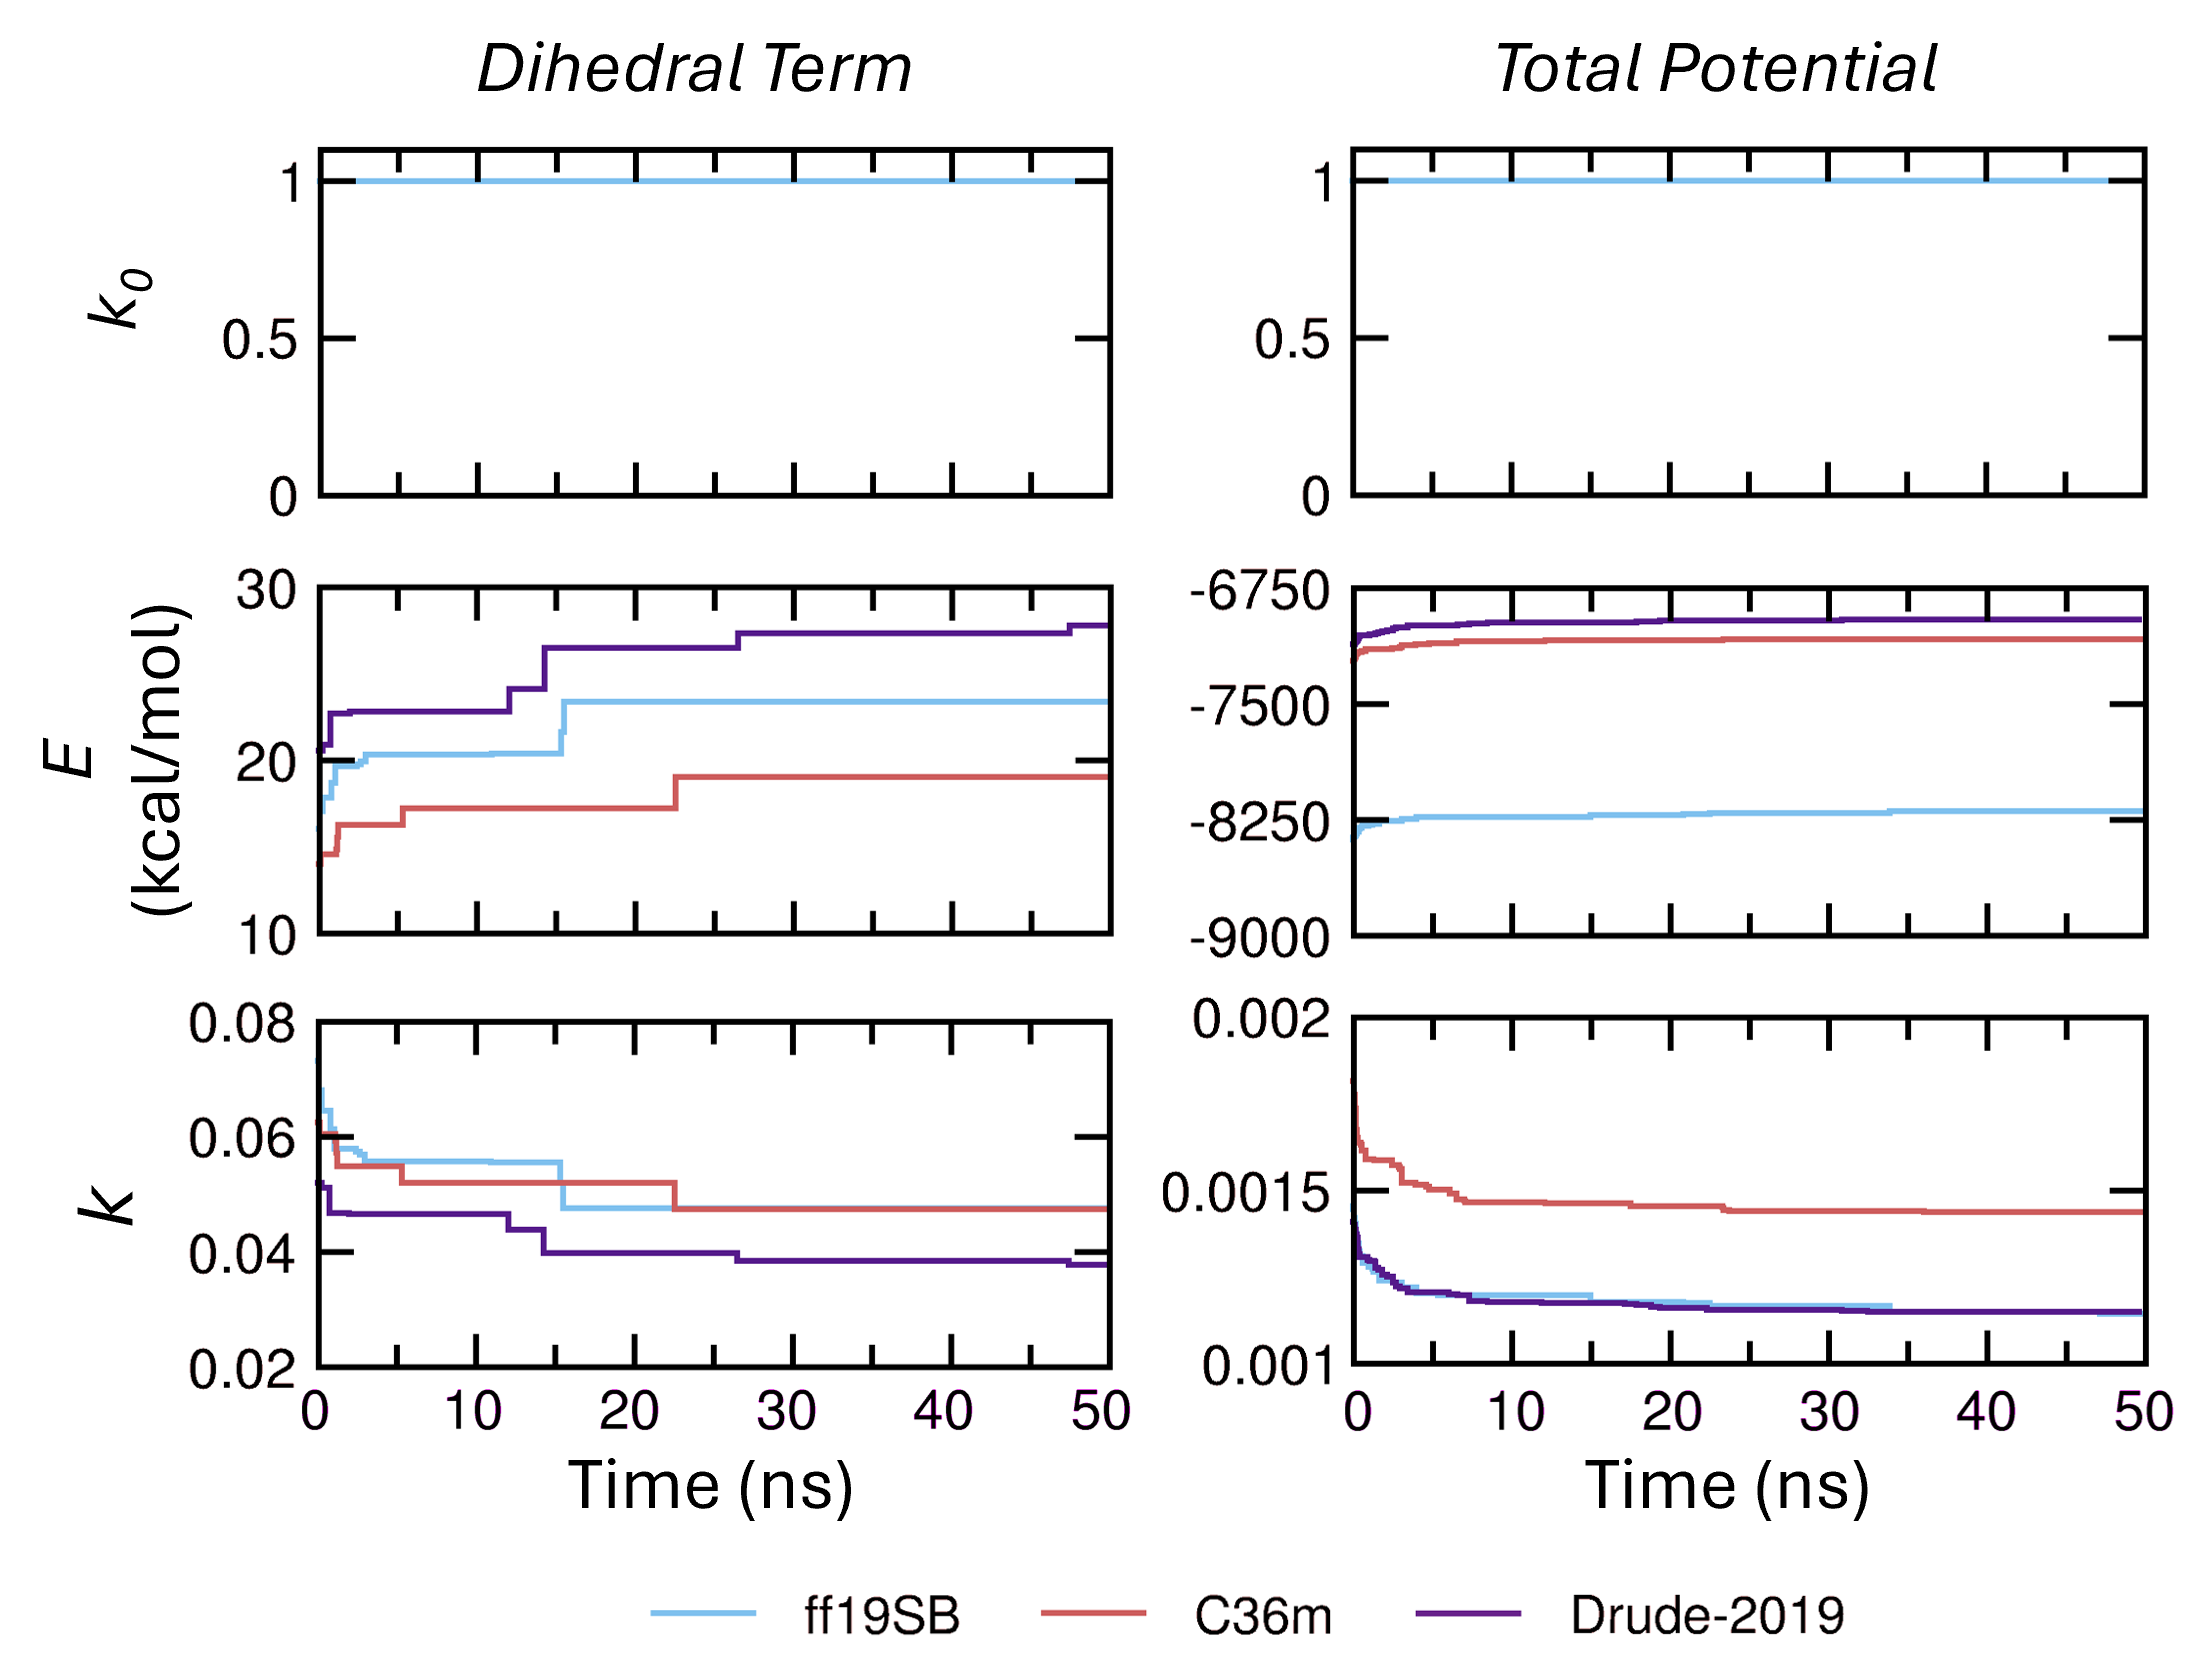
\includegraphics[width=\columnwidth]{main_figs/equil_conv.png}
    \caption{GaMD parameters as a function of time during equilibration.}
    \label{fig:equil_conv_alad}
\end{figure}

Ideally, $k_{0}$ will reach 1 during equilibration, indicating that the system has the highest dynamic acceleration, however, we note that even when $k_{0}$ reaches 1, $E$ may still be increasing. As $E$ is directly involved in the boost equation shown in Eq.~\ref{eqn:boost}, we suggest also monitoring $E$ during equilibration to ensure that the system reaches its highest possible energy. Such an outcome is indicated by $E$ leveling off towards the end of the equilibration steps. As shown in Figure~\ref{fig:equil_conv_alad}, each force field reached the highest acceleration indicated by $k_{0}$ reaching a value of 1, however, there are differences in the time series of $E$ for each FF. The differences in system potential energy are due to the inherent differences in the  potential energy terms in each force field. The time series also show how quickly the system reaches a converged $E$ for the dihedral term with ff19SB and C36m, whereas Drude may need additional time to reach its maximum possible energy. Use of a polarizable force field with GaMD is still relatively new, thus the time required to equilibrate should be studied further. A particularly important point is that the Drude force field has inherently slower kinetics than C36m and most nonpolarizable force fields. This difference arises from the more realistic diffusion of the SWM4-NDP water model~\cite{lamoureux_swm4_2006} compared to the (CHARMM-modified) TIP3P model~\cite{jorgensen_tip3p_1983,durell_solv_1994,neria_activate_1996} used in conjunction with C36m. This same trend is shown with the total potential energy but is less obvious due to the scale of energy differences across force fields.

The time series for $k$ is also shown as it is involved in the boost calculation, however, we do not regularly monitor $k$ as it is inversely correlated to $E$ and thus exhibits the same behavior as $E$.

\subsubsection{Production} \label{ss:tutorial_prod}
Once the system has reached equilibration convergence, the output files can then be used to set up the GaMD production run. In \texttt{prod}, we will need the system topology, \texttt{ala.parm7} for ff19SB, \texttt{ala.c36.psf} for C36m, or \texttt{ala.drude.psf} for Drude. A few different files from the end of equilibration will be required for production. The coordinate file (\texttt{gamd\_equil.coor}), the atomic velocity file (\texttt{gamd\_equil.vel}), and the file containing the box size (\texttt{gamd\_equil.xsc}), should all be copied to the production folder. Additionally, the file containing the GaMD parameters from the last step of equilibration, \texttt{gamd\_equil.gamd}, will also need to be copied to this directory. The job submission script  (\texttt{sub\_gamd\_prod.sh}) and the production run template file (\texttt{md.template}) will also need to be present in this directory. 

Only slight changes are required to the the file, \texttt{md.template} which serves as our template for the GaMD production input scripts. All prep, conventional, and equilibration steps should be set to 0 and \texttt{accelMDGRestart} should be turned on to read in the GaMD restart file from equilibration. The production phase is set to run in strides of 10 ns or 10000000 steps for Drude and 5000000 steps for C36m and ff19SB. To do so, the template file will be used to generate nearly identical input files for each stride, named \texttt{md.*.in}, with * indicating the stride number. The generated input files will be populated with variables such as <BASE>, <BASENAME>, and <CURR>, which are specified in the \texttt{sub\_gamd\_prod.sh}. <BASE> will be populated by the system name the user chooses, while <BASENAME> and <CURR> are automatically populated based on the current stride. <BASENAME> will be set to \texttt{gamd\_equil} if the current stride is 1, otherwise will be set to the system name, force field, and previous stride number. For example, the <BASENAME> for stride 2 of the Drude alanine dipeptide system would be \texttt{ala.drude.2}. Finally, <CURR> is set to the current stride number that is being simulated. These variables will be used as the prefixes for output files that will be read in to begin the next stride. Once the topology and coordinate files, submission script,  template files are in the working directory, submit the production run submission script, e.g. via SLURM:

%\bigskip
%\texttt{\$ sbatch sub\_gamd\_prod.sh}
\begin{lstlisting}[style=MyBash]
$ sbatch sub_gamd_prod.sh
\end{lstlisting}

For each stride, the coordinate, velocity, box size, and GaMD restart files will be output in a manner similar to equilibration. All the integral boost information required for reweighting will be found in the output files named \texttt{md.*.out}.

\subsection{Constructing the Free Energy Profile}
Once the production simulations have reached the desired simulation length, we can start to extract the information required to reweight our simulations and obtain a free energy profile. The following subsections will detail this process. All steps described here can be carried out using the \texttt{gamd\_postprocess.sh} script from our GitHub. 

\subsubsection{Collating Weights and Collective Variables}
All important GaMD information is printed to the output files, named \texttt{md.*.out}, with the * indicating the numeric stride of production. For reweighting, we first need to combine the data from all strides together into one file, which we will name \texttt{gamd\_md.log} file. If using the command line, this task can be completed using the \texttt{cat} command.

\begin{lstlisting}[style=MyBash]
$ cat md.{1..50}.out > gamd_md.log
\end{lstlisting}

Using a command described in the PyReweighting tutorial (\url{https://mccammon.ucsd.edu/computing/amdReweighting/}), we can extract the boost potential values for each step and calculate the weights in $k_{B}T$ using the equipartition theorem, $E_{kinetic} = \frac{3}{2}RT$ (see below, \$6/(0.001987*298)).

\begin{lstlisting}[style=MyBash]
$ grep "ACCELERATED MD" gamd_md.log | grep -v "GAUSSIAN" | grep -v "ACTIVE" | awk '{print $6/(0.001987*298)" " $4 " " $6 " "$8}' > raw_weights.dat
\end{lstlisting}

This command will created a file called \texttt{raw\_weights.dat} (Listing ~\ref{weights}), containing the boost in $k_{B}T$ (column 1) alongside the associated simulation step (\$4, column 2), the boost in kcal/mol of that step (\$6, column 3), and the average boost (\$8, column 4). 


\begin{lstlisting}[label=weights, caption=raw\_weights.dat, basicstyle=\small, backgroundcolor=\color{light-gray}]
13.3554   0 	   7.90805 	 7.90805
16.0597   10000    9.50935 	 7.69249
13.2625	  20000    7.85307 	 7.5384
14.7218   30000    8.71715 	 8.167
14.4863   40000    8.57769 	 7.78162
16.9263   50000    10.0225 	 8.13965
19.0174   60000    11.2607 	 8.59088
13.4737   70000    7.97811 	 8.4957
\end{lstlisting}

Note that if you are running production in strides like this tutorial, the simulation steps in the weight file will range from 0 to 10000000 for a single stride, then start over at step 0 for the next stride. To use this file for reweighting, the steps will need to be renumbered continuously from 0 through the final step of the simulation. For our simulations of 500 ns, we use a Python script called \texttt{fix\_time\_gamd.py} that will read the \texttt{raw\_weights.dat} file and renumber the steps to produce a usable \texttt{weights.dat} file for reweighting. 

The next step is to generate the CVs. Since this tutorial is focused on alanine dipeptide, we chose to use a 2-dimensional reweighting scheme using the backbone $\phi$ and $\psi$ torsions. Since the output files for production are written in strides of 10 ns, to analyze our systems, we need to generate one trajectory file for the entire simulation. NAMD writes the trajectories in DCD format, so we use the \texttt{catdcd} program to compile them all.

\begin{lstlisting}[style=MyBash]
$ catdcd -o full.dcd ala.19sb.{1..50}.dcd
\end{lstlisting}

This command will generate a single DCD-formatted trajectory file named \texttt{full.dcd} that can then be used for subsequent analysis. For all systems, water was stripped and each system was oriented to remove global rotation and translation of the alanine dipeptide. For Drude and C36m, a in-house script (\texttt{orient.inp}) was used to orient the systems with the CHARMM program. We then generated $\phi$ and $\psi$ angles using another CHARMM script. For ff19SB, an in-house script was used to orient with CPPTRAJ and a Python script was used to generate $\phi$ and $\psi$ using AmberTools22. To ensure we can have a functional CV file for reweighting, both $\phi$ and $\psi$ must be in the same file (\texttt{cv.dat}) containing only two columns, the first of which contains the time series of $\phi$ values and the second column contains the time series of $\psi$ values.

At this point, we have a file containing the boost values (\texttt{weights.dat}) and a file containing our CVs (\texttt{cv.dat}) for the full simulations. Both the weight file and the CV file should be copied to the local workstation (if running the simulations on a remote server), if not done so already. In our simulations, we created directories specifically for each alanine dipeptide system with a \texttt{reweight} directory for all our reweighting work. As a reminder, the majority of this post-processing can be done using the \texttt{gamd\_postprocess.sh}.   

\subsubsection{Reweighting} \label{ss:tutorial_reweight} 
 All scripts required to perform reweighting and generate free energy surfaces are in the GitHub repository. These scripts execute all steps besides generating the boost distributions and are executed using the \texttt{gen\_fes\_converge.sh} script. Before beginning reweighting, it is beneficial to check the anharmonicity of $\Delta{V}$ to ensure the applied boosts follow a Gaussian, or normal, distribution. To do so, use the \texttt{make\_dist.py} in the GitHub repository to generate a probability density distributions using the boost in kcal/mol found in the third column of \texttt{weights.dat}. 

\bigskip
\begin{lstlisting}[style=MyBash]
$ python make_dist.py -data weights.dat -col 2 -out dist_boost.dat
\end{lstlisting}

Once generated, \texttt{dist\_boost.dat} can be visualized using XmGrace or any other 2D plotting utility. For each of our systems, we generated the boost distributions, which are shown in Figure~\ref{fig:dist_boost}.

\begin{figure}[h]
    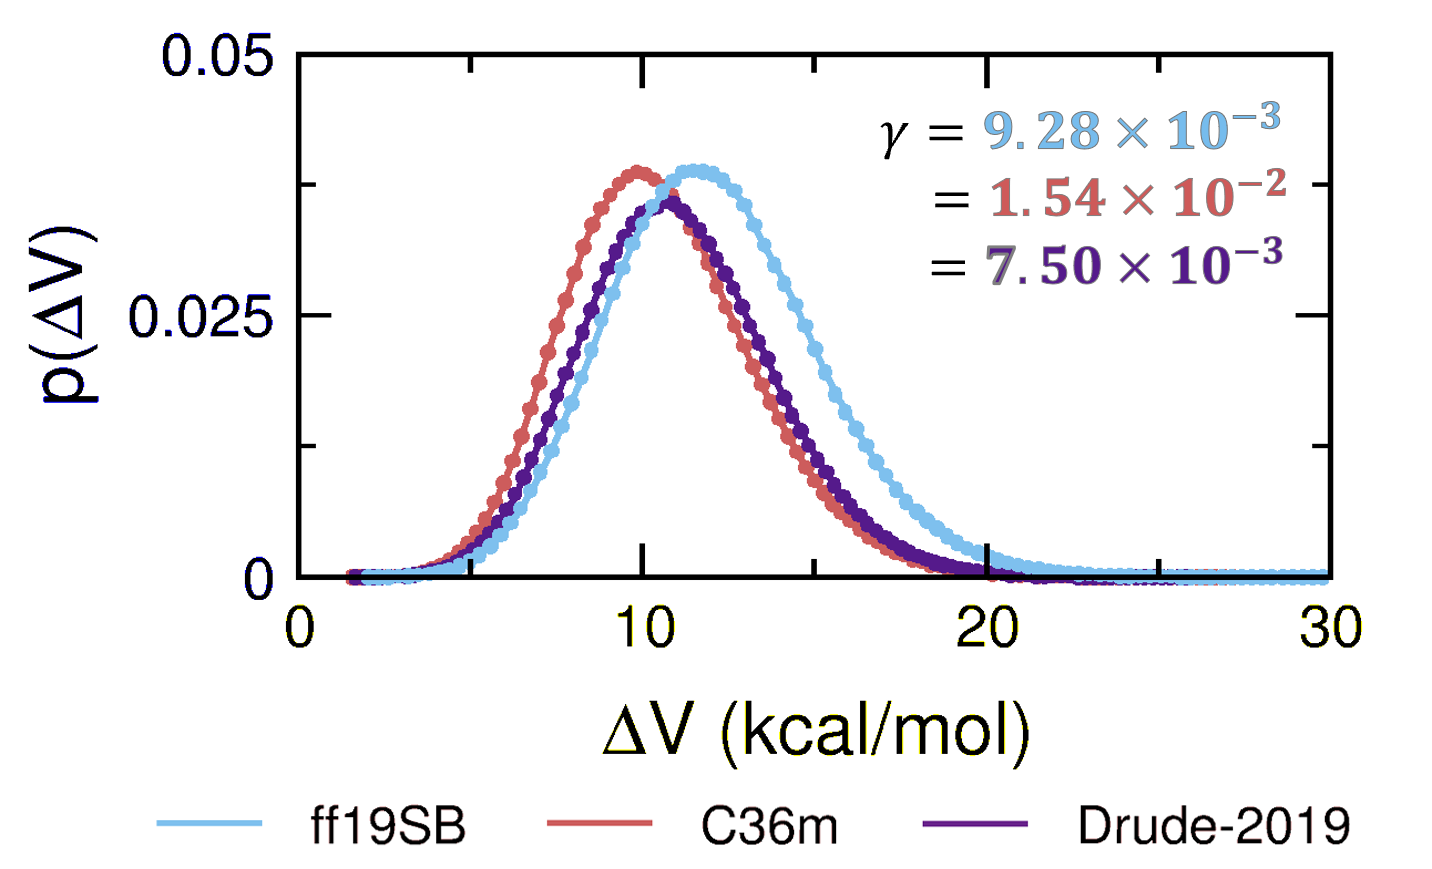
\includegraphics[width=\columnwidth]{main_figs/dist_boost_allffs.png}
    \caption{Distribution of boost potential for alanine dipeptide systems.}
    \label{fig:dist_boost}
\end{figure}

In general, each of the systems produced a distribution of boost potentials that resembles a normal distribution centered around similar boost values. This graph can be complemented by the anharmonicity values, $\gamma$, which are also shown in Figure~\ref{fig:dist_boost}. Anharmonicity can be used to characterize the distribution of the applied boost potentials and act as a checkpoint for GaMD simulations. All $\gamma$ values are close to 0, indicating a Gaussian-shaped distribution in each simulation, irrespective of the force field used. The anharmonicity is an output of reweighting, which will be detailed below.

To begin reweighting, clone the PyReweighting repository into the \texttt{reweight} directory. A detailed explanation of the files within the toolkit can be found in Section~\ref{sec:workflow}. For this tutorial, we will focus on the files for reweighting in two dimensions: \texttt{PyReweighting\_2D.py} and \texttt{reweight-2D.sh}. In general, the \texttt{PyReweighting-2D.py} script will not need to be opened or edited, so it does not need to be in the \texttt{reweight} directory. However, \texttt{reweight-2D.sh} should be placed in the \texttt{reweight} directory in case it needs to be edited for a specific system. The user will also need to specify the path to the \texttt{PyReweighting-2D.py} script. 

Start by creating a conda environment (see \url{https://docs.conda.io/projects/conda/en/latest/user-guide/tasks/manage-environments.html}) that is equipped with all Python packages necessary to execute \texttt{PyReweighting-2D.py}. At the top of \texttt{PyReweighting-2D.py}, there is a section listing the required packages for installation. Specify the Python version to be 3.10 in the conda environment, then install the packages. In our environment, we used SciPy version 1.9.1, NumPy version 1.23.3, and Matplotlib version 3.6.1. We have also provided our environment in the form of a YAML file on GitHub. All versions stated here have been tested for this tutorial but other versions may also work. 

Once the environment is set up, activate it to preparing to run the reweighting. The \texttt{reweight-2d.sh} script contains a section at the top to set variables required to reweight. These values can either read in via the command line or changed directly in the file, as shown in Listing~\ref{re_variables}. First, set the path to the \texttt{PyReweighting-2D.py} script. This path will depend on where the user decides to save the \texttt{pyreweighting} directory. Then, set \texttt{Emax} to represent the maximum possible free energy value obtained from the calculations. We set \texttt{Emax} to 100 in our script but we tested a range of values for \texttt{Emax}, finding that it had little to no impact on the resulting PMF profile. \texttt{Emax} essentially acts as a safeguard in the instance that a histogram bin has no occupancy (zero probability), which would otherwise result in an undefined (infinite) energy value. Next, set \texttt{cutoff} to 10, which requires that each bin contains at least 10 frames to be considered for reweighting. The x- and y-values will be used for \texttt{-Xdim} and \texttt{-Ydim} and act as the total possible range of $\phi$ and $\psi$ values for the dipeptide. Here, we use a range from -180 to 181 as Python will incorporate all values between -180 and 181 but excluding 181. The CV values will be separated into bins depending on the width of each bin, which can be adjusted using \texttt{binx} and \texttt{biny}. The Python script will then assign these values to the arguments \texttt{-discx} and \texttt{-discy}. We suggest systematically evaluating the distribution of data points sampled over the range of values along the CVs, such as the $\phi$ and $\psi$ angles, and setting the bin size accordingly. Here, we chose 15 degrees as the width since it is a factor of 180, a common reporting convention for dihedral angles. In our experience, it is often necessary to test multiple bin sizes to identify which one best represents the data. The CV file, \texttt{cv.dat}, is then specified using \texttt{data}. Finally, temperature, \texttt{T}, is set at 298 K to match our simulation temperature. 


\bigskip
\begin{lstlisting}[label=re_variables, caption=Reweight-2d.sh, basicstyle=\small, backgroundcolor=\color{light-gray}]
#!/bin/bash
dir_codes=/home/pyreweighting/
Emax=100
cutoff=10
Xmin=-180
Xmax=181
Ymin=-180
Ymax=181
binx=15
biny=15
data="cv.dat"
T=298
\end{lstlisting}

The only other aspect of the script to check and modify is the name of the weight file. The default file name from the PyReweighting Toolkit is \texttt{weights.dat} so if the user's file is named something else, this will need to be edited to read in the correct weight file. Once the \texttt{reweight-2d.sh} is edited it can be executed via the command line (e.g., for Bash):

\begin{lstlisting}[style=MyBash]
$ bash reweight-2d.sh
\end{lstlisting}

This command will initialize the reweighting process and print a progress report to the terminal and a log file named \texttt{reweight\_variable.log}. The minimum PMF values for cumulant expansion to the first, second, and third orders will all be printed so one can identify the lowest energy that is then used to normalize all the PMF values such that the lowest value is zero. The total anharmonicity of $\Delta{V}$ is also output in this progress report when \texttt{amd\_dV} reweighting is used:

\begin{lstlisting}[label=anharm, basicstyle=\small, backgroundcolor=\color{light-gray}]
Anharmonicity of all dV = 0.009284925479752903
\end{lstlisting}

In this tutorial, we are focused primarily on the outputs of reweighting using cumulant expansion through the \texttt{-job amdreweight\_CE}. The outputs are all shown in Listing~\ref{ce_outputs}.

\bigskip
\begin{lstlisting}[label=ce_outputs, caption=Reweighting Outputs, basicstyle=\small, backgroundcolor=\color{light-gray}]
pmf-2D-c3-cv_500.dat-reweight-discx15-discy15.xvg
pmf-2D-c2-cv_500.dat-reweight-discx15-discy15.xvg
pmf-2D-c1-cv_500.dat-reweight-discx15-discy15.xvg
pmf-2D-cv_500.dat-reweight-CE2-discx15-discy15.png
pmf-2D-cv_500.dat-noweight-discx15-discy15.xvg
pmf-2D-cv_500.dat-noweight-discx15-discy15.png
\end{lstlisting}

For cumulant expansion to the second order, we will focus on the values in \texttt{pmf-2D-c2-cv\_500.dat-reweight-discx15\\-discy15.xvg}. The file is structured with the first CV, $\phi$, in the first column and the second CV, $\psi$, in the second column (Listing~\ref{pmf_c2}). The values of $\phi$ and $\psi$ are in discrete increments of 15 degrees from -180 to 180 as we specified in \texttt{reweight-2d.sh}. The corresponding PMF value is in the third column. Put another way, this file shows that for every ($\phi$, $\psi$) pair, there is a corresponding PMF value.

\bigskip
\begin{lstlisting}[label=pmf_c2, caption=pmf-2D-c2-cv\_500.dat-reweight-discx15-discy15.xvg, basicstyle=\small, backgroundcolor=\color{light-gray}]
#RC1    RC2     PMF(kcal/mol)

@    xaxis  label "RC1"
@    yaxis  label "RC2"
@TYPE xy
-180.0  -180.0  6.511680581400153
-180.0  -165.0  7.268263041332778
-180.0  -150.0  11.271196453661494
-180.0  -135.0  11.324540393639706
-180.0  -120.0  4.952376113451482
-180.0  -105.0  7.193065613889537
-180.0  -90.0   5.495317166801527
-180.0  -75.0   4.618741411987148
-180.0  -60.0   6.06630454462983
-180.0  -45.0   5.397685481887759
-180.0  -30.0   5.901996954706036
-180.0  -15.0   5.781848121714702
-180.0  0.0     7.741654368167012
...
\end{lstlisting}

\begin{figure*}[t]
    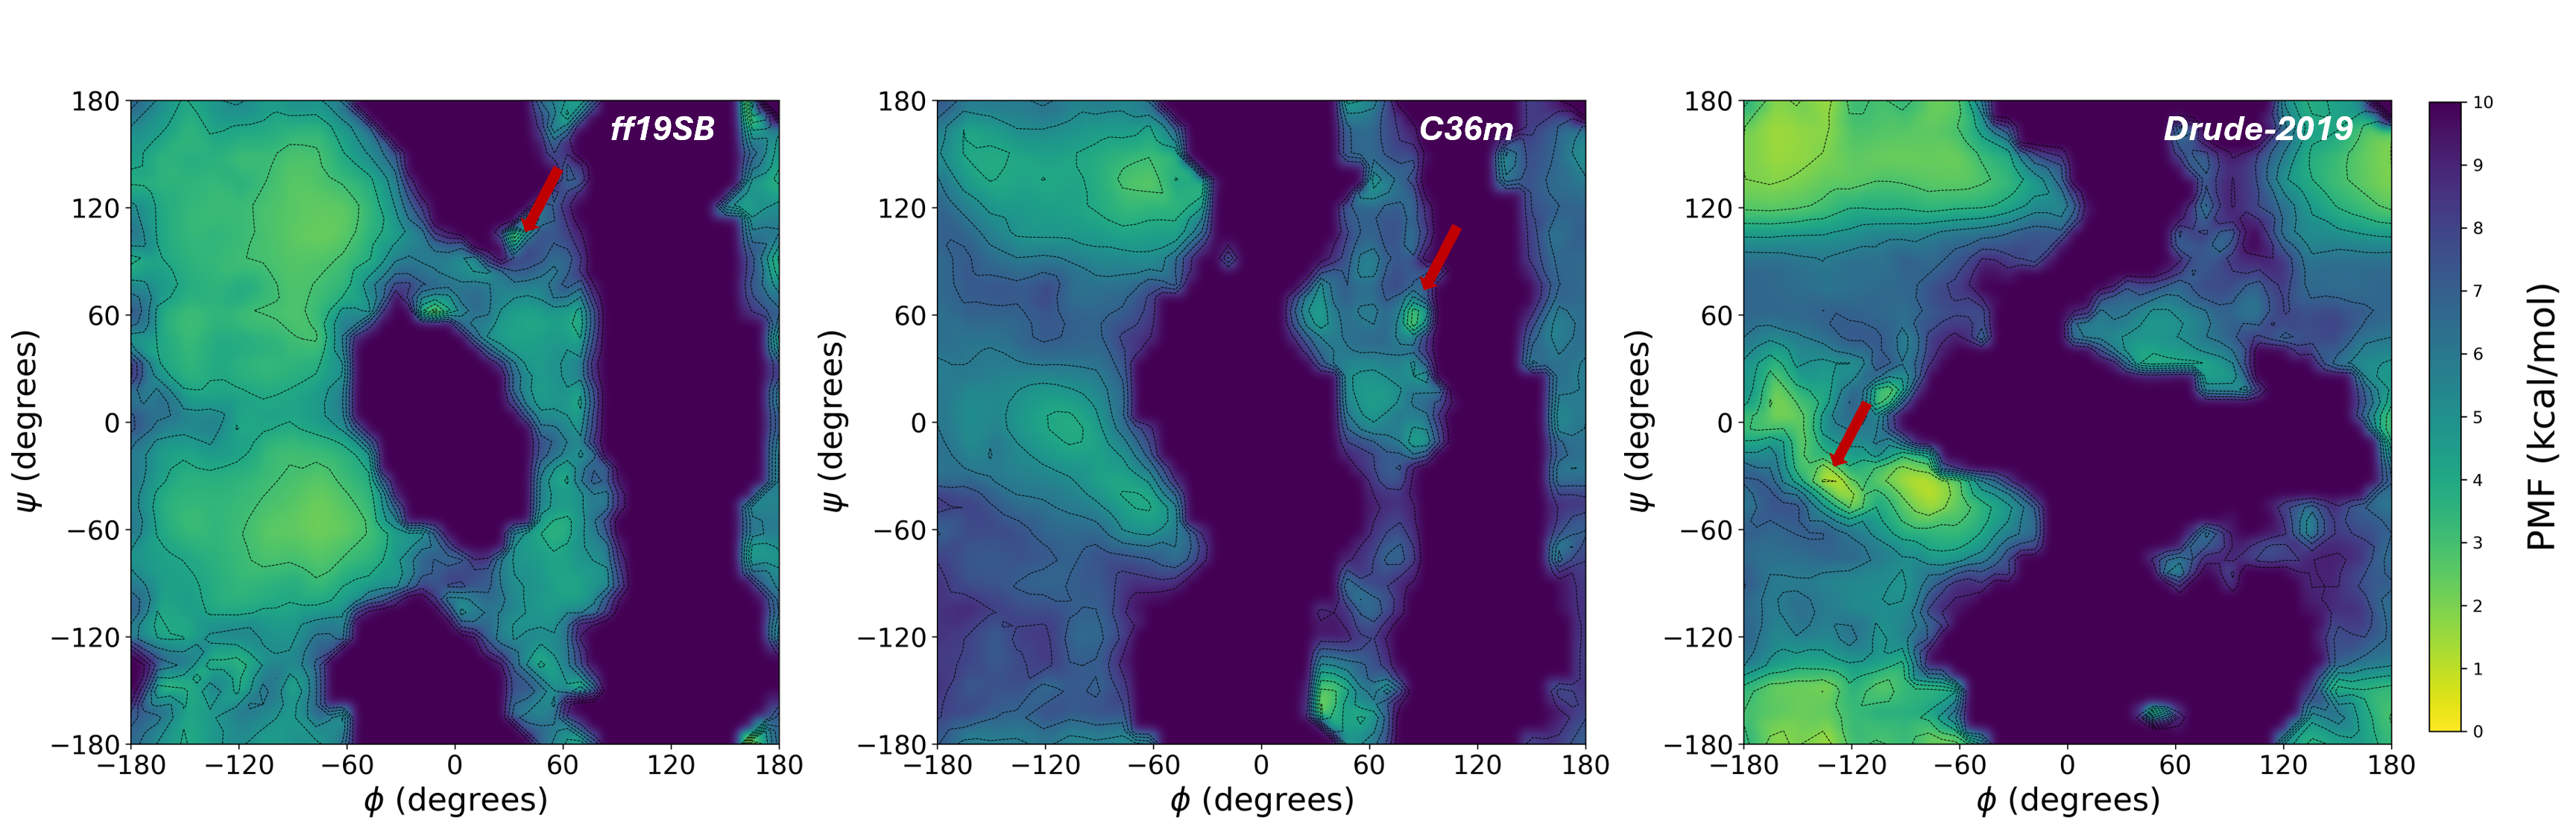
\includegraphics[scale=0.68]{main_figs/alad_allfes_500.png}
    \caption{FES for all alanine dipeptide systems. The global minimum in each surface is indicated by a red arrow.}
    \label{fig:alad_allffs}
\end{figure*}

As noted above, the reweighting script normalizes the PMF values such that the global minimum is zero. The lowest free energy value that was printed to the terminal earlier is the offset factor. For example, \texttt{pmf\_min-c2 = -22.22813527319225} for our ff19SB system, so 22.22813527319225 is added to every PMF value to generate the normalized range of values. Note that these data will be used to produce a Ramachandran plot in the next section, which represents a continuous range of $\phi$ and $\psi$ values. Plotting the PMF values now will result in a seemingly ``missing'' row and column corresponding to ($\phi$,$\psi$) = (180, 180) degrees. We included a Python script (\texttt{fix\_phipsi.py}) in the GitHub repository that will read through the PMF file and copy $\phi$ and $\psi$ values from -180 to 180. Doing so will generate the symmetry inherent in Ramachandran plots. 

\begin{lstlisting}[style=MyBash]
$ python fix_phipsi.py pmf-2D-c2-cv_500.dat-reweight-discx15- \
discy15.xvg fix_pmf_c2.xvg
\end{lstlisting}

The \texttt{fix\_phipsi.py} script generates a new file called \texttt{fix\_pmf\_c2.xvg}, which can be used to render the FES and identify the free energy minima. 

\subsubsection{Plotting the Surface and Identifying Minima}
Since we installed the \texttt{matplotlib} package into our conda environment, we can continue working within this environment to generate FES. We have included an example Python script, \texttt{plot\_csv.py}, to generate the FES shown in Figure~\ref{fig:alad_allffs}. A complete description of the contents of the script is beyond the scope of this tutorial but we will highlight lines that may be useful to edit depending on the system being analyzed. 

\begin{description}
    \item[zcutoff] Conceptually similar to $Emax$ from reweighting, the script resets any PMF value above zcutoff to the zcutoff value. In this example, we are using 10.
    \item[contour\_levels] Here you can specify what PMF values you what to outline with contour lines. For this example, we chose PMF values of 0, 2, 4, 6, 8, and 10 kcal/mol.
    \item[x and y axes] Specifies formatting of the x- and y-axes such as tick marks, label sizes, and label ranges.
\end{description}

The script can be run by specifying the input file, an output image name, and a zcutoff value. 

\begin{lstlisting}[style=MyBash]
$ python plot_csv.py fix_pmf_c2.xvg fes_ff19sb_500.png 10
\end{lstlisting}

This command creates a PNG image file that can be qualitatively analyzed to localize the minima. However, we can also determine the exact x- and y-coordinates on our FES the correspond to these minima. We have provided a \texttt{find\_minima\_2D.py} script that will take user inputs including the PMF file name, output file name, and a PMF threshold, which will be used as search criteria to find any PMF below the specified threshold.

\begin{lstlisting}[style=MyBash]
$ python find_minima_2d.py pmf-2D-c2-cv_500.dat-reweight-discx15- \
discy15.xvg minima.dat 2
\end{lstlisting}

This command generates a file that designates the minima based on the PMF and the associated $\phi$ and $\psi$ values to match the FES, as shown in Listing~\ref{minima}. 

\begin{lstlisting}[label=minima, caption=minima.dat, basicstyle=\small, backgroundcolor=\color{light-gray}]
# phi     psi     PMF 
-15.0     60.0      0.001988476330325284
30.0      105.0     0.0
75.0      -150.0    0.45605829164178147
165.0     -180.0    0.5940885730567551
\end{lstlisting}

Thus, it is possible to identify the exact location of the global minimum and other local minima, and the associated PMF in kcal/mol. The FES for all three alanine dipeptide systems are shown in Figure~\ref{fig:alad_allffs}. The force fields yielded slight differences. For ff19SB and C36m, the global minima are located within the left-handed $\alpha$-helix region. Typically, this region is not sampled, but due the small methyl side chain of alanine, it experiences fewer steric clashes and ultimately can adopt a more diverse set of dihedral angles, which may explain the location of the global minima in these systems. With the Drude force field, the surface has a global minimum in the $\alpha$-helical region, which is expected due to the tendency for this force field to sample $\alpha_R$ configurations at slightly higher frequencies than C36m~\cite{lin_further_2020}.

\subsection{Considerations}
Throughout the GaMD process, there are a few places of consideration that can potentially alter the system's sampling and FES. We have included a few considerations below that we experienced while setting up our simulations.

\subsubsection{Statistical Window size} 
The \texttt{accelMDGStatWindow} keyword is specified in the input scripts for equilibration and production and determines how often statistical averaging for the potential energies is performed and how often the boost is recalculated. Conventionally, this value should be around four times the total number of particles in the system. For the alanine dipeptide systems, this convention would suggest a window between 10000 and 20000 steps would be appropriate. For the tutorials, we used a value of 10000 for each of our systems, but we performed an additional simulation using 20000 to compare the resulting FES. The surfaces for ff19SB with \texttt{accelMDGStatWindow} values of 10000 and 20000 steps are shown in Figure~\ref{fig:binstatw}. The general shape of the surfaces differ only slightly although the surface arising from the simulation with \texttt{accelMDGStatWindow} set to 20000 is systematically higher by 3-4 kcal/mol than that of  the system with \texttt{accelMDGStatWindow} set to 10000. Applying \texttt{accelMDGStatWindow} 20000 did have a lower energy minimum prior to normalization during reweighting, which could be the cause of the shift in PMF. Additionally, these differences could be a result of under- or over-sampling of the same state across these two systems and may therefore not be directly linked to the specified value of \texttt{accelMDGStatWindow}. 

\begin{figure*}[h]
    \includegraphics[scale=0.68]{main_figs/bin_statw_comp.png}
    \caption{Comparison of the free energy surfaces for ff19SB simulations using \texttt{accelMDGStatWindow} values of 10000 and 20000.}
    \label{fig:binstatw}
\end{figure*}

\subsubsection{Bin Width} 
Bin width is specified during the reweighting process and will impact the way the data are binned, thus potentially altering the location of the global minimum on the reweighted FES. We compared the use of different bin sizes by reweighting using \texttt{-discx} and \texttt{-discy} set to 6 and 15 (Figure~\ref{fig:binstatw}). Bin size will be based on the amount of CV data collected as well as the range of the data values. Previously published GaMD studies using alanine peptide used a bin size of 6$^{\circ}$.\cite{miao_gaussian_2015} In our approach, such a small bin size was not appropriate to visualize the surfaces (Figure ~\ref{fig:binstatw}, top and bottom left), most likely because we saved fewer frames than the previously published studies, implying that the bin width may be directly connected to the number of data points saved during the simulation.

\subsubsection{Bin Cutoff}
Another consideration that may be dependent upon the number of frames is the bin cutoff. This cutoff is specified during the reweighting process to ensure undersampled bins do not dominate the free energy surfaces. The value specified using \texttt{cutoff} sets a minimum number of frames required for that bin to be used during reweighting, any bin containing a number of frames less than the specified value is not considered during reweighting. Thus, different cutoff values can result in FES with different global minima (Figure ~\ref{fig:binstatw}).

\subsubsection{Simulation Convergence} 
An integral component of running MD simulations is ensuring that the system sampled as much of the conformational landscape as theoretical possible. In the case of GaMD, we evaluated the convergence of the data used to produce our FES. We generated surfaces across intervals of 50, 100, 200, 300, 400, and 500 ns to determine if the features of the FES were still changing. These surfaces for ff19SB, C36m, and Drude-2019 are shown in Figures~\ref{fig:19sb_conv} -~\ref{fig:drude_conv}. As mentioned in Section~\ref{ss:tutorial_reweight}, the \texttt{gen\_convergence\_fes.py} script in our GitHub repository will generate all these surfaces.

\begin{figure*}
    \includegraphics[scale=0.62]{main_figs/19sb_conv.png}
    \caption{Time evolution of the FES for ff19SB simulations.}
    \label{fig:19sb_conv}
\end{figure*}

\begin{figure*}
    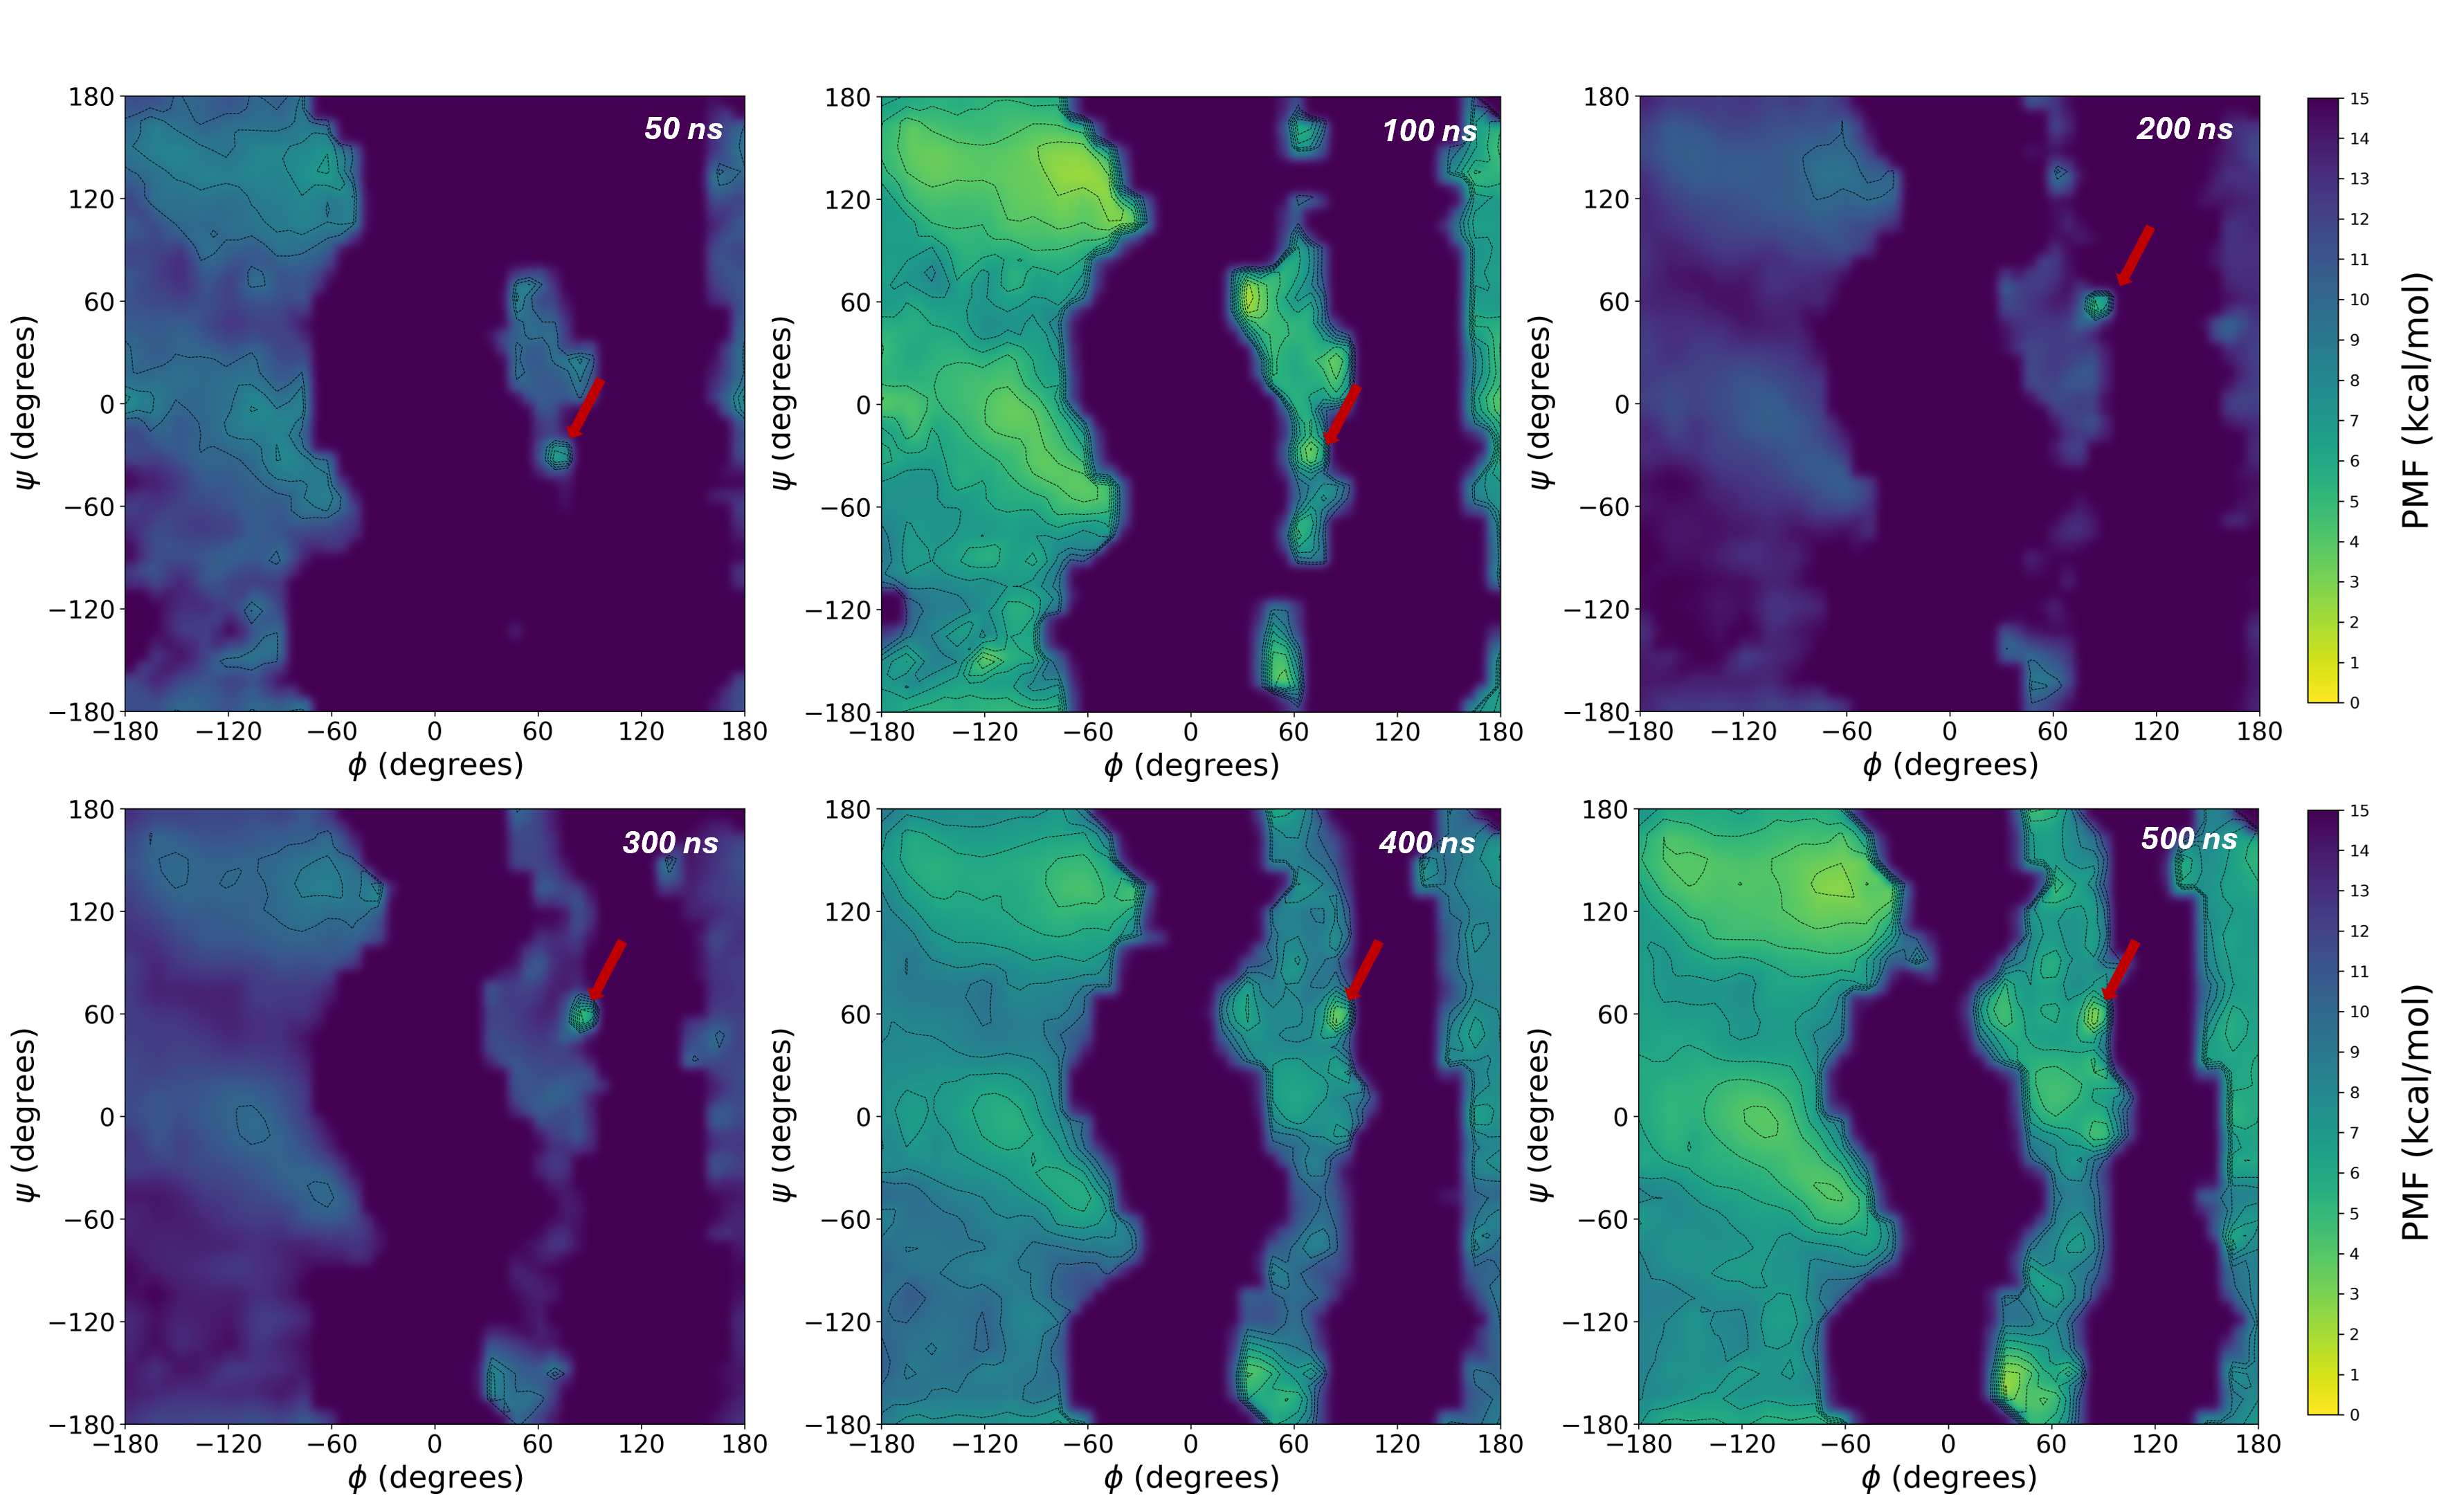
\includegraphics[scale=0.62]{main_figs/c36_conv.png}
    \caption{Time evolution of the FES for C36m simulations.}
    \label{fig:c36_conv}
\end{figure*}

\begin{figure*}[h]
    \includegraphics[scale=0.60]{main_figs/drude_conv.png}
    \caption{Time evolution of the FES for Drude-2019 simulations.}
    \label{fig:drude_conv}
\end{figure*}


\subsection{Summary and Review of Objectives}
In this tutorial, the user has been guided through the process of completing a GaMD simulation. To review, the objectives for this tutorial were as follows: 

\begin{enumerate}
    \item Identify key elements of the theory underlying GaMD simulations
    \item Prepare and run GaMD simulations using NAMD
    \item Reweight and analyze the GaMD free energy profiles using the PyReweighting toolkit
\end{enumerate}

The first step towards achieving these objectives was the setup of conventional MD and GaMD equilibration in which the type of boost (total, dihedral, or dual) was specified, along with the number of simulation steps. The output files obtained from GaMD and NAMD were reviewed, with special attention given to \texttt{gamd\_equil.out}, which contains all the statistical information used to calculate the boost and determine the extent of equilibration convergence, and \texttt{gamd\_equil.gamd}, which contains the threshold energy to be used for production. The system was then set up for GaMD production, during which the boost for each step was calculated based on the difference between finalized threshold energy from equilibration and the system potential energy at that step. The tutorial concluded with the generation and visualization of free energy profiles using $\phi$ and $\psi$ dihedrals for the alanine dipeptide system.


\section{Author Contributions}
HM Michel developed and wrote the tutorial. MD Polêto and JA Lemkul provided guidance for tutorial development. 

\section{Other Contributions}
We thank all members of the Lemkul Lab for helpful discussions and feedback. We specifically thank Laura I. Gil Pineda, Rebekah J. Fogarty, and Patrick C. Gilles for providing detailed feedback and extensive testing throughout the development of the tutorials. Additionally, we would like to thank Aakash Saha and Pablo R. Arantes for insightful discussions about the GaMD process in AMBER.

\section{Potentially Conflicting Interests}

The authors declare no conflicting interests.

\section{Funding Information}

This work was supported by the National Institutes of Health (grant R35GM133754 to JAL) and USDA-NIFA (project VA-160211 to JAL).

% BIBLIOGRAPHY
\bibliography{gamdtutorial}

\end{document}